%%%% utfprpb.tex, 2019/12/03
%%%% Copyright (C) 2020 Vinicius Pegorini (vinicius@utfpr.edu.br)
%%
%% This work may be distributed and/or modified under the conditions of the
%% LaTeX Project Public License, either version 1.3 of this license or (at your
%% option) any later version.
%% The latest version of this license is in
%%   http://www.latex-project.org/lppl.txt
%% and version 1.3 or later is part of all distributions of LaTeX version
%% 2005/12/01 or later.
%%
%% This work has the LPPL maintenance status `maintained'.
%%
%% The Current Maintainer of this work is Vinicius Pegorini.
%%
%% This work consists of the files utfprpb.cls, utfprpb.tex, and
%% utfprpb-dados.tex.
%%
%% A brief description of this work is in readme.md.

%% Classe e opções de documento
\documentclass[%% Opções
%% -- Opções da classe memoir --
  12pt,%% Tamanho da fonte: 10pt, 11pt, 12pt, etc.
  a4paper,%% Tamanho do papel: a4paper (A4), letterpaper (carta), etc.
  % fleqn,%% Alinhamento das equações à esquerda (comente para alinhamento centralizado)
  % leqno,%% Numeração das equações no lado esquerdo (comente para lado direito)
  oneside,%% Impressão dos elementos textuais e pós-textuais: oneside (anverso) ou twoside (anverso e verso, se mais de 100 p.)
  openright,%% Impressão da primeira página dos capítulos: openright (anverso), openleft (verso) ou openany (anverso e verso)
%% -- Opções da classe abntex2 --
  sumario = abnt-6027-2012,%% Formatação do sumário: tradicional (estilo tradicional) ou abnt-6027-2012 (norma ABNT 6027-2012)
  chapter = TITLE,%% Títulos de capítulos em maiúsculas (comente para desabilitar)
  % luiz - comentar section para ser minusculo
  %section = TITLE,%% Títulos de seções secundárias em maiúsculas (comente para desabilitar)
  % subsection = TITLE,%% Títulos de seções terciárias em maiúsculas (comente para desabilitar)
  % subsubsection = TITLE,%% Títulos de seções quartenárias em maiúsculas (comente para desabilitar),
%% -- Opções da classe utfprpgtex --
  pretextualoneside,%% Impressão dos elementos pré  -textuais: pretextualoneside (anverso) ou pretextualtwoside (anverso e verso)
  fontetimes,%% Fonte do texto: fontetimes (times), fontearial (arial) ou fontecourier (courier)
  % vinculoscoloridos,%% Cores nos vínculos (citações, arquivos, links, url, etc.) (comente para desabilitar)
  semrecuonosumario,%% Remoção do recuo dos itens no sumário (comente para adição do recuo, se estilo tradicional)
  usemakeindex,%% Compilação de glossários e índices utilizando makeindex (comente para desabilitar)
  % legendascentralizadas,%% Alinhamento das legendas centralizado (comente para alinhamento à esquerda)
  %aprovacaoestiloppg,%% Folha de aprovação do programa de pós-graduação no estilo do PPG (comente para estilo padrão)
  pardeassinaturas,%% Assinaturas na folha de aprovação em até duas colunas (comente para em uma única coluna)
  % linhasdeassinaturas,%% Linhas de assinaturas na folha de aprovação (comente para remover as linhas)
%% -- Opções do pacote babel --
  english,%% Idioma adicional para hifenização
  french,%% Idioma adicional para hifenização
  spanish,%% Idioma adicional para hifenização
  brazil,%% Idioma principal do documento (último da lista)
]{utfpr}%% Classe utfpr


%% Pacotes carregados nas classes:
%%   memoir: abstract, appendix, array, booktabs, ccaption, chngcntr, chngpage, dcolumn, delarray, enumerate, epigraph, framed,
%%           ifmtarg, ifpdf, index, makeidx, moreverb, needspace, newfile, nextpage, parskip, patchcmd, setspace, shortvrb, showidx,
%%           tabularx, titleref, titling, tocbibind, tocloft, verbatim, verse.
%%   memoir (similares): crop, fancyhdr, geometry, sidecap, subfigure, titlesec.
%%   abntex2: babel, bookmark, calc, enumitem, ifthen, hyperref, textcase.
%%   utfprpgtex: abntex2cite, ae, algorithmic, amsmath, backref, breakurl, caption, cmap, color, eepic, epic, epsfig, etoolbox,
%%               fancyhdr, fix-cm, fontenc, glossaries, graphics, graphicx, helvet, hyphenat, indentfirst, inputenc, lastpage,
%%               morewrites, nomencl, sfmath, sistyle, substr, times, xtab.


%% Pacotes adicionais (\usepackage[options]{package})
\usepackage{bigdelim, booktabs, colortbl, longtable, multirow}%% Ferramentas para tabelas
\usepackage{amssymb, amstext, amsthm, icomma}%% Ferramentas para linguagem matemática
\usepackage{pifont, textcomp, wasysym}%% Símbolos de texto
\usepackage{lipsum}				% para geração de dummy text
\usepackage{subfig}             % para adicionar figuras lado a lado no texto                    
\usepackage{pdfpages}           % para adicionar documentos pdf ao trabalho
\usepackage{xspace}


% luiz: primeira letra maiúscula
% solução 1
%\usepackage{stringstrings}
%\newcommand{\firstcap}[1]{\caselower[e]{#1}\capitalize{\thestring}}

% solução 2 - não usei essa
% \usepackage[utf8]{inputenc}
% \usepackage{datatool-base}
% \usepackage{mfirstuc}

% Formatação do título da seção - primeira letra caixa alta e o resto em caixa baixa.
% \usepackage[explicit]{titlesec}
% \usepackage{lipsum}
% \titleformat{\section}{\normalfont}{\thesection}{1em}{\textbf{\firstcap{#1}}} % funciona mas apenas para o título da seção e não para o sumário (a configuração do sumário está mais para baixo

% luiz: define o underline colorido.
% https://github.com/abntex/abntex2-contrib/blob/master/customizacoes/pucminas/abntex2-pucminas.sty
% acabei não usando o black e o coloruline da solução do link

\usepackage[normalem]{ulem} % para o underline colorido na seção quaternária
\renewcommand*{\cftsubsubsectionfont}{\normalfont\uline} % underline no sumário
\setsubsubsecheadstyle{\ABNTEXsubsubsectionfont\ABNTEXsubsubsectionfontsize\ABNTEXsubsubsectionupperifneeded\uline} %underline no título da subsubsection

% luiz: bibliografia - opções

%% Comandos personalizados (\newcommand{name}[num]{definition})
\newcommand{\cpp}{\texttt{C$++$}}%% C++
\newcommand{\latex}{\LaTeX\xspace}%% LaTeX
\newcommand{\ds}{\displaystyle}%% Tamanho normal das equações
\newcommand{\bsym}[1]{\boldsymbol{#1}}%% Texto no modo matemático em negrito
\newcommand{\mr}[1]{\mathrm{#1}}%% Texto no modo matemático normal (não itálico)
\newcommand{\der}{\mr{d}}%% Operador diferencial
\newcommand{\deri}[2]{\frac{\der #1}{\der #2}}%% Derivada ordinária
\newcommand{\derip}[2]{\frac{\partial #1}{\partial #2}}%% Derivada parcial
\newcommand{\pare}[1]{\left( #1 \right)}%% Parênteses
\newcommand{\colc}[1]{\left[ #1 \right]}%% Colchetes
\newcommand{\chav}[1]{\left\lbrace #1 \right\rbrace}%% Chaves
\newcommand{\sen}{\operatorname{sen}}%% Operador seno
\newcommand{\senh}{\operatorname{senh}}%% Operador seno hiperbólico
\newcommand{\tg}{\operatorname{tg}}%% Operador tangente
\newcommand{\tgh}{\operatorname{tgh}}%% Operador tangente hiperbólico
\newcommand{\seqref}[1]{Equação~\eqref{#1}}%% Referência de uma única equação
\newcommand{\meqref}[1]{Equações~\eqref{#1}}%% Referência de múltiplas equações
\newcommand{\citep}[1]{\cite{#1}}%% Atalho para citação implícita
\newcommand{\citet}[1]{\citeonline{#1}}%% Atalho para citação explícita
\newcommand{\citepa}[1]{(\citeauthor{#1})}%% Atalho para citação implícita (somente autor)
\newcommand{\citeta}[1]{\citeauthoronline{#1}}%% Atalho para citação explícita (somente autor)
\newcommand{\citepy}[1]{(\citeyear{#1})}%% Atalho para citação implícita (somente ano)
\newcommand{\citety}[1]{\citeyear{#1}}%% Atalho para citação explícita (somente ano)

\newcommand{\fonteTexto}[1]{\renewcommand{\familydefault}{#1}}

% Define o caminho das figuras
\graphicspath{{figuras/}}

% Define a fonte ara helvet que é uma fonte similar à Arial, se for usar a Arial tem que mudar o compilador para XeLaTex, mas ai tem que arrumar os erros: https://latex.org/forum/viewtopic.php?t=25998
%\usepackage{helvet}
%\renewcommand{\familydefault}{\sfdefault}
%\usepackage{times} % para fonte time new roman
%\usepackage{pslatex} % ou essa aqui...

%\usepackage{titlesec}

%% Configuração de glossário
% \usepackage[portuguese]{nomencl}
% \usepackage[nogroupskip,nonumberlist,nopostdot,nohypertypes={acronym}]{glossaries}
% \makenoidxglossaries
\usepackage{glossaries}
\makeglossaries

% para siglas em português
\newcommand{\siglaPt}[2]
{
 \newglossaryentry{#1}{
  name=#1,
  description={#2},
  first={#2 (#1)},
  long={#2}
 }  
}

% para siglas de língua estrangeira, nessas a descrição longa fica em itálico.
\newcommand{\siglaIt}[2]
{
 \newglossaryentry{#1}{
  name=#1,
  description={\textit{#2}},
  first={\textit{#2} ({#1})},
  long={\textit{#2}}
 }  
}

%% luiz - para fazer os avisos
\usepackage{tcolorbox}

% use para criar caixas de avisos, pode ser utilizado para fazer anotações de tarefas indicadas pelo orientador/banca.
% \caixa{Atenção}{texto...}
\newcommand{\caixa}[2]{
\begin{tcolorbox}[colback=red!5!white,colframe=red!45!white, title = #1, fonttitle=\bfseries]
#2
\end{tcolorbox}
}






%% Arquivo de dados do modelo de documento LaTeX para produção de trabalhos acadêmicos da UTFPR
%%%% utfprpb-dados.tex, 2019/12/03
%%%% Copyright (C) 2020 Vinicius Pegorini (vinicius@utfpr.edu.br)
%%
%% This work may be distributed and/or modified under the conditions of the
%% LaTeX Project Public License, either version 1.3 of this license or (at your
%% option) any later version.
%% The latest version of this license is in
%%   http://www.latex-project.org/lppl.txt
%% and version 1.3 or later is part of all distributions of LaTeX version
%% 2005/12/01 or later.
%%
%% This work has the LPPL maintenance status `maintained'.
%%
%% The Current Maintainer of this work is Vinicius Pegorini.
%% Updated by:
%% - Marco Aurélio Graciotto Silva;
%% - Rogério Aparecido Gonçalvez;
%% - Luiz Arthur Feitosa dos Santos.
%%
%% This work consists of the files utfpr.cls, main.tex, and
%% variaveis.tex.
%%
%% A brief description of this work is in readme.txt.

%% Documento
%% Luiz: Define a fonte do texto da monografia
\fonteTexto{\sfdefault} % utilize \rmdefault para Times New Roman ou \sfdefault para Arial
\TipoDeDocumento{Trabalho de Conclusão de Curso de Graduação}%% Tipo de documento: "Tese", "Dissertação" ou "Trabalho de Conclusão de Curso de Graduação", "Estágio Supervisionado"
\NivelDeFormacao{Bacharelado}%% Nível de formação: "Doutorado", "Mestrado", "Bacharelado" ou "Tecnólogo" - ATENÇÃO, isso será utilizado para alterar a formatação do trabalho, pois pode haver formatações distintas dependendo o nível/tipo de trabalho.


%% luiz
% Template LaTex criado pelo Departamento Acadêmico de Computação (DACOM)
% da Universidade Tecnológica Federal do Paraná - Campus Campo Mourão (UTFPR-CM)
% Criado e alterado pelos professores:
% - Marco Aurélio Graciotto Silva
% - Rogério Aparecido Gonçalvez
% - Luiz Arthur Feitosa dos Santos
% Esse template utiliza a licença CC BY:
% Esta licença permite que outros distribuam, remixem, adaptem e criem a partir deste trabalho, mesmo para fins comerciais, desde que atribuam o devido crédito pela criação original.
% https://creativecommons.org/licenses/by/4.0/deed.pt_BR

% Dados do curso. Caso seja BCC:
\program{}
\programen{Undergradute Program in Computer Science}
\degree{Bacharel}
\degreearea{Engenharia Eletrônica}
% Caso seja TSI:
% \program{Curso Superior de Tecnologia em Sistemas para Internet}
% \programen{Undergradute Program in Tecnology for Internet Systems}
% \degree{Tecnólogo}
% \degreearea{Tecnologia em Sistemas para Internet}


% Dados da disciplina. Escolha uma das opções e a descomente:
% TCC1:
%\goal{Proposta de Trabalho de Conclusão de Curso de Graduação}
%\course{Trabalho de Conclusão de Curso 1}
% TCC2:
 \goal{Trabalho de Conclusão de Curso de Graduação}
 \course{Trabalho de Conclusão de Curso 2}


% Dados do TCC (precisa alterar)
\author{JOSE BARRETO DOS SANTOS JUNIOR}  % Seu nome
\authorbib{Silva, João da} % Seu nome para referência bibliográfica (Sobrenome, Nome)
\title{DESENVOLVIMENTO DE PROTÓTIPO PARA CONTROLE DE ACESSO UTILIZANDO RECONHECIMENTO FACIAL} % Título do trabalho
\titleen{Development of a prototype for access control using facial recognition} % Título traduzido para inglês
\advisor{Eduardo Giometti Bertogna} % Nome do orientador. Lembre-se de prefixar com "Prof. Dr.", "Profª. Drª.", "Prof. Me." ou "Profª. Me."}
% Se não houver corientador, comente a linha a baixo
%\coadvisor{} % Nome do coorientador, caso exista. Caso não exista, comente a linha.
\depositshortdate{2023} % Ano em que depositou este documento
\approvaldate{ /novembro/2023}

% Dados do curso que não precisam de alteração
\university{Universidade Tecnológica Federal do Paraná}
\universityen{Federal University of Technology -- Paraná}
\universitycampus{Campus Campo Mourão}
\universityunit{Departamento Acadêmico de Computação}
\address{CAMPO MOURÃO}
\addressen{Campo Mourão, PR, Brazil}
\documenttype{Monografia}
\documenttypeen{Monograph}
\degreetype{Graduação}

\evalboardmember{Prof. Dr. Lucas Ricken Garcia}{Avaliador(a) 1}{UTFPR}
\evalboardmember{Prof. Dr. Osmar Tormena Junior}{Avaliador(a) 2}{UTFPR}
\evalboardmember{Prof. Dr. Eduardo Giometti Bertogna}{Orientador(a)}{UTFPR}
%\evalboardmember{Nome completo e por extenso do Membro 4}{Título (especialização, mestrado, doutorado}{Nome completo e por extenso da instituição a qual possui vínculo}

%% Palavras-chave e keywords
%% ATENÇÃO - você deve indicar a quantidade de palavras chaves para o template LaTeX utilizar o pontuação correta!
\NumeroDePalavrasChave{3}%% Número de palavras-chave (máximo 5)
\PalavraChaveA{Reconhecimento facial}%% Palavra-chave A
\PalavraChaveB{Controle de acesso}%% Palavra-chave B
\PalavraChaveC{Biometria}%% Palavra-chave C
%\PalavraChaveD{Palavra-chave 4}%% Palavra-chave D
%\PalavraChaveE{Palavra-chave 5}%% Palavra-chave E

%% ATENÇÃO - você deve indicar a quantidade de keywords para o template LaTeX utilizar o pontuação correta!
\NumeroDeKeywords{3}%% Número de keywords (máximo 5)
\KeywordA{Facial recognition}%% Keyword A
\KeywordB{Access control}%% Keyword B
\KeywordC{Biometry}%% Keyword C
%\KeywordD{Keyword 4}%% Keyword D
%\KeywordE{Keyword 5}%% Keyword E


% É obrigatório o uso de uma licença Creative Commons (CC) nos trabalhos de TCC pelos cursos ligados a DACOM da UTFPR-CM.
% Veja: http://portal.utfpr.edu.br/biblioteca/trabalhos-academicos/docentes/procedimento-de-entrega-graduacao

% Sendo assim, escolha com o seu orientador uma das licenças CC a seguir: 

% CC BY: Esta licença permite que outros distribuam, remixem, adaptem e criem a partir deste trabalho, mesmo para fins comerciais, desde que atribuam o devido crédito pela criação original. Essa é a menos restritiva.
\licenca{ccby}

% CC BY CA: Esta licença permite que outros remixem, adaptem e criem a partir deste trabalho, mesmo para fins comerciais, desde que atribuam o devido crédito e que licenciem as novas criações sob termos idênticos.
%\licenca{ccbysa}

% CC BY ND: Esta licença permite a redistribuição, comercial e não comercial, desde que o trabalho seja distribuído inalterado e no seu todo, com crédito ao autor.
%\licenca{ccbynd}

% CC BY NC: Esta licença permite que outros remixem, adaptem e criem a partir deste trabalho para fins não comerciais, e embora os novos trabalhos tenham de atribuir o devido crédito e não possam ser usados para fins comerciais, os trabalhos derivados não têm que serem licenciados sob os mesmos termos.
%\licenca{ccbync}

% CC BY NC SA: Esta licença permite que outros remixem, adaptem e criem a partir deste trabalho para fins não comerciais, desde que atribuam ao autor o devido crédito e que licenciem as novas criações sob termos idênticos.
%\licenca{ccbyncsa}

% CC BY NC ND: Esta licença só permite que outros façam download do trabalho e o compartilhe desde que atribuam crédito ao autor, mas sem que possam alterá-los de nenhuma forma ou utilizá-los para fins comerciais. Essa é a mais restritiva.
%\licenca{ccbyncnd}

% Deixar sem licença - isso é aplicado apenas aos trabalhos que não são obrigados a ter licença. Na duvida verifique isso com o seu orientador e professor responsável pelo TCC. Para deixar o texto sem licença deixe o comando licença em brando ou deixe comentado.
%\licenca{}
% by DACOM/UTFPR-CM%% Realize as modificações pertinentes no arquivo "utfprpb-dados.tex"

%% Ferramenta para criação de índices
\makeindex%% Não comente esta linha

%% Ferramenta para criação de glossários
\makeglossaries%% Não comente esta linha
%%%% LISTA DE ABREVIATURAS E SIGLAS 
%%
%% Relação, em ordem alfabética, das abreviaturas (representação de uma palavra por meio de alguma(s) de sua(s) sílaba(s) ou
%% letra(s)), siglas (conjunto de letras iniciais dos vocábulos e/ou números que representa um determinado nome) e acrônimos
%% (conjunto de letras iniciais dos vocábulos e/ou números que representa um determinado nome, formando uma palavra pronunciável).
%%
%% Este arquivo para definição de abreviaturas, siglas e acrônimos é utilizado com a opção "glossaries" (pacote)

%% Abreviaturas: \abreviatura{rótulo}{representação}{definição}

\abreviatura{art.}{art.}{Artigo}
\abreviatura{cap.}{cap.}{Capítulo}
\abreviatura{sec.}{sec.}{Seção}

%% Siglas: \sigla{rótulo}{representação}{definição}

\sigla{abnt}{ABNT}{Associação Brasileira de Normas Técnicas}
\sigla{cnpq}{CNPq}{Conselho Nacional de Desenvolvimento Científico e Tecnológico}
\sigla{eps}{EPS}{\textit{Encapsulated PostScript}}
\sigla{pdf}{PDF}{Formato de Documento Portátil, do inglês \textit{Portable Document Format}}
\sigla{ps}{PS}{\textit{PostScript}}
\sigla{utfpr}{UTFPR}{Universidade Tecnológica Federal do Paraná}

%% LEIA:

%% Para usar o \gls, você deve colocar a sigla aqui em \sigla

%% ADICIONAR SIGLAS: Quando você inclui alguma sigla, pode ser necessário compilar umas duas vezes para essa aparecer na lista de siglas.

%% ATENÇÃO REMOVER SIGLAS: se você remover a sigla do seu texto (não for usar mais), você deve comentar essa aqui e remover os \gls{} dessa sigla (se não vai ficar aparecendo a sigla na lista). Em caso de ERRO, quando o LaTeX informa que você ainda tem a sigla no texto, mesmo que não tenha. Você deve limpar o cache - no OverLeaf, clique no erro, vá:
%  ->view error
%%   ->(role para baixo, até o final)
%%     ->e clique em Clear cached files


%% Acrônimos: \acronimo{rótulo}{representação}{definição}
%\acronimo{gimp}{Gimp}{Programa de Manipulação de Imagem GNU, do inglês \textit{GNU Image Manipulation Program}}
%% Entradas da lista de abreviaturas e siglas - Comente para remover este item
%%%% GLOSSÁRIO
%%
%% Relação de palavras ou expressões técnicas de uso restrito ou de sentido obscuro, utilizadas no texto, acompanhadas das
%% respectivas definições.

%% Entradas do glossário: \newglossaryentry{rótulo}{informações da entrada}

\newglossaryentry{pai}{%% Informações da entrada
  name        = {pai},
  plural      = {pais},
  description = {um exemplo de entrada pai que possui subentradas (entradas filhas)}
}

\newglossaryentry{componente}{%% Informações da entrada
  name        = {componente},
  plural      = {componentes},
  parent      = {pai},
  description = {um exemplo de uma entrada componente, subentrada da entrada chamada \gls{pai}}
}

\newglossaryentry{filho}{%% Informações da entrada
  name        = {filho},
  plural      = {filhos},
  parent      = {pai},
  description = {um exemplo de uma entrada filha (subentrada) da entrada chamada \gls{pai}. Trata-se de uma entrada irmã da entrada chamada \gls{componente}}
}

\newglossaryentry{equilibrio}{%% Informações da entrada
  name        = {equilíbrio da configuração},
  see         = [veja também]{componente},
  description = {uma consistência entre os \glspl{componente}}
}

\newglossaryentry{tex}{%% Informações da entrada
  name        = {\TeX},
  sort        = {TeX},
  description = {é um sistema de tipografia criado por Donald E. Knuth}
}

\newglossaryentry{latex}{%% Informações da entrada
  name        = {\latex},
  sort        = {LaTeX},
  description = {um conjunto de macros para o processador de textos \gls{tex}, utilizado amplamente para a produção de textos matemáticos e científicos devido à sua alta qualidade tipográfica}
}

\newglossaryentry{bibtex}{%% Informações da entrada
  name        = {Bib\TeX},
  sort        = {BibTeX},
  parent      = {latex},
  description = {um software de gerenciamento de referências para a formatação de listas de referências. A ferramenta Bib\TeX\ é normalmente usada em conjunto com o sistema de preparação de documentos do \gls{latex}}
}

\newglossaryentry{abntex2}{%% Informações da entrada
  name        = {\abnTeX},
  sort        = {abnTeX2},
  see         = {latex},
  description = {uma suíte para \gls{latex} que atende os requisitos das normas da Associação Brasileira de Normas Técnicas (ABNT) para elaboração de documentos técnicos e científicos brasileiros, como artigos científicos, relatórios técnicos, trabalhos acadêmicos como teses, dissertações, projetos de pesquisa e outros documentos do gênero}
}

\newglossaryentry{utfprpbtex}{%% Informações da entrada
  name        = {\utfprpbtex},
  sort        = {UTFPRPBTeX},
  see         = {latex},
  parent      = {abntex2},
  description = {uma suíte para \gls{latex}, baseada na suíte \gls{abntex2}, que atende os requisitos das normas definidas pela Universidade Tecnológica Federal do Paraná (UTFPR), Câmpus Pato Branco, para elaboração de trabalhos acadêmicos}
}
%% Entradas do glossário - Comente para remover este item

%% Ferramenta para criação de nomenclaturas
\makenomenclature%% Não comente esta linha

%% Início do documento
\begin{document}%% Não comente esta linha

%% Formatação de páginas de elementos pré-textuais
\pretextual%% Não comente esta linha

%% Capa
%\incluircapa%% Comente para remover este item
\coverpageone

%% Folha de rosto (* coloca a ficha bibliográfica no verso)
%\incluirfolhaderosto*%% Comente para remover este item
\coverpagetwo

%% Ficha catalográfica (teses e dissertações)
%\incluirfichacatalografica%% Comente para remover este item

%% Errata
%%%%% ERRATA
%%
%% Lista dos erros ocorridos no texto, seguidos das devidas correções.

\begin{errata}%% Ambiente errata
\begin{table*}[htb]%% Ambiente table
\begin{tabularx}{\textwidth}{|l|l|X|X|}%% Ambiente tabularx
\hline
\textbf{Página(s)}         & \textbf{Linha(s)} & \textbf{Onde se lê} & \textbf{Leia-se}         \\ \hline
\pageref*{errata:capitulo} & 4, 9-11, 14-16    & capítulo(s)         & seção(ões) primária(s)   \\ \hline
\pageref*{errata:secao}    & 12-16             & seção(ões)          & seção(ões) secundária(s) \\ \hline
\pageref*{errata:subsecao} & 16                & subseção(ões)       & seção(ões) terciária(s)  \\ \hline
\end{tabularx}
\end{table*}
\end{errata}
%% Comente para remover este item

%% Folha de aprovação
%\incluirfolhaaprovacao
\approvalpage
%\incluirfolhadeaprovacao%% Para adicionar no formato de texto
%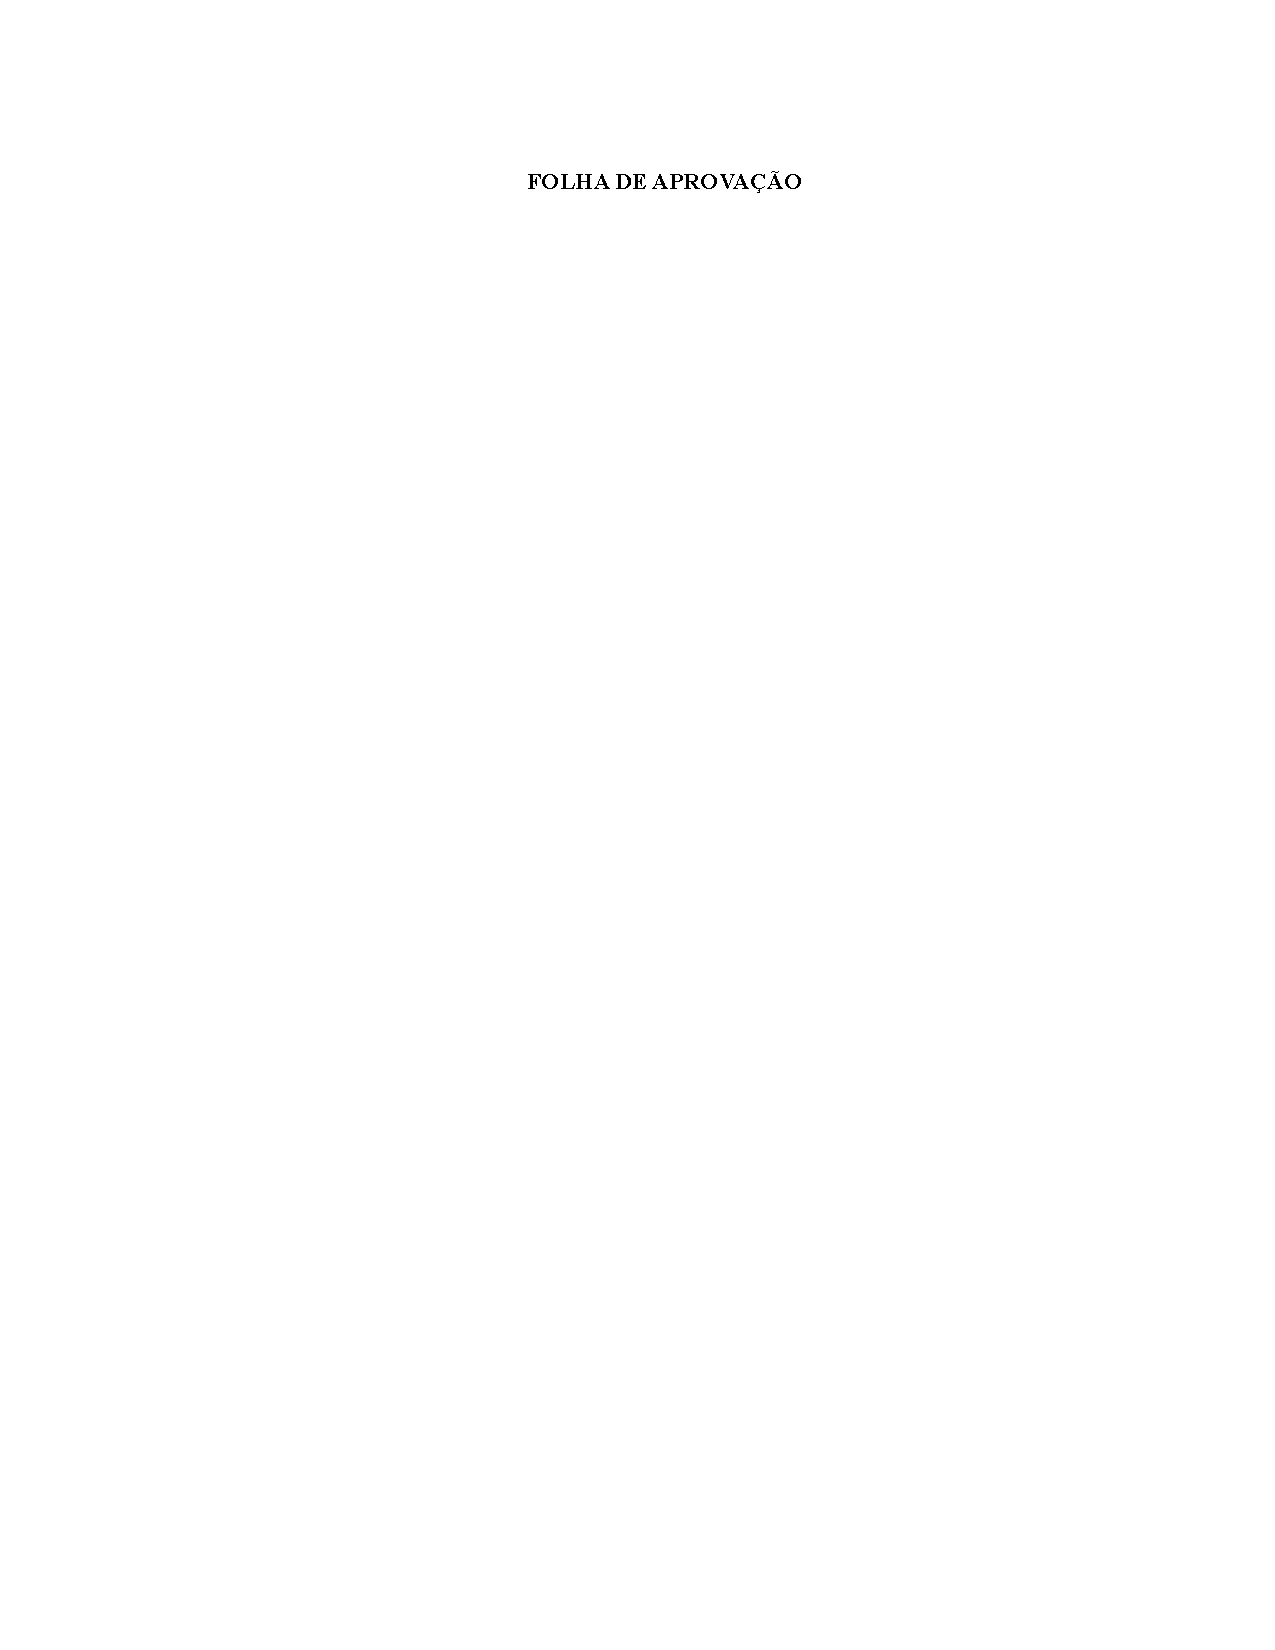
\includepdf[scale=1.0,pages=1]{./PreTexto/folha-aprovacao.pdf} % para adicionar o pdf enviado pelo professor apenas substitua o documento folha-aprovacao.pdf dentro da pasta PreTexto

%% Dedicatória
%%%%% DEDICATÓRIA
%%
%% Texto em que o autor presta homenagem ou dedica seu trabalho.

\begin{dedicatoria}%% Ambiente dedicatoria

Espaço destinado à dedicatória (elemento opcional).
Folha que contém o oferecimento do trabalho à determinada pessoa ou pessoas. Exemplo:

Dedico este trabalho à minha família, pelos momentos de ausência.

\end{dedicatoria}
%% Comente para remover este item

%% Agradecimentos
%%%% AGRADECIMENTOS
%%
%% Texto em que o autor faz agradecimentos dirigidos àqueles que contribuíram de maneira relevante à elaboração do trabalho.

\begin{agradecimentos}%% Ambiente agradecimentos

Agradeço ao meu orientador Prof. Dr. Eduardo Bertonha, pelo apoio e tempo dedicado durante esta trajetória, onde durante a elaboração do trabalho sempre compartilhou conhecimento e experiência.

Aos meus colegas de sala, à minha esposa, e à meus pais, pois sempre confiaram e acreditaram em mim e sem o apoio deles seria mais difícil conseguir superar esse desafio. 

\end{agradecimentos}
%% Comente para remover este item

%% Epígrafe
%%%%% EPÍGRAFE
%%
%% Texto em que o autor apresenta uma citação, seguida de indicação de autoria, relacionada com a matéria tratada no corpo do
%% trabalho.

\begin{epigrafe}%% Ambiente epigrafe
Primeira Lei: Um robô não pode ferir um ser humano ou, por omissão, permitir que um ser humano sofra algum mal. Segunda Lei: Um robô deve obedecer as ordens que lhe sejam dadas por seres humanos, exceto nos casos em que tais ordens contrariem a Primeira Lei. Terceira Lei: Um robô deve proteger sua própria existência desde que tal proteção não entre em conflito com a Primeira e Segunda Leis (ASIMOV, Isaac, 1950). 

(elemento opcional)
\end{epigrafe}
%% Comente para remover este item

%% Resumo
%%%% RESUMO
%%
%% Apresentação concisa dos pontos relevantes de um texto, fornecendo uma visão rápida e clara do conteúdo e das conclusões do
%% trabalho.

\begin{resumoutfpr}%% Ambiente resumoutfpr

A biometria, em sistemas de segurança, tem sido amplamente utilizada devido sua 
confiabilidade, podendo ser empregada para acessar contas bancárias, autenticação de 
estabelecimentos, pagamento em dispositivos móveis, controle de acesso, etc. 
Dentre as biometrias disponíveis, o reconhecimento facial se destaca pela sua 
praticidade e por ser uma das biometrias mais estudadas e utilizadas. 
Podendo ser aplicada sem a necessidade de um contato físico. Diante disso, 
o presente estudo, visa o desenvolvimento de um protótipo de 
reconhecimento facial para controle e autenticação de acesso. Para essa finalidade, 
será utilizado um dispositivo ESP32-CAM, que será responsável por capturar e 
classificar as imagens em tempo real. Sendo essas imagens processadas por intermédio 
de algorítimos de detecção e reconhecimento facial.
\end{resumoutfpr}
%% Comente para remover este item

%% Abstract
%%%% ABSTRACT
%%
%% Versão do resumo para idioma de divulgação internacional.

\begin{abstractutfpr}%% Ambiente abstractutfpr
    Facial recognition is applied in various technologies such as cell phone unlocking, establishment authentication, means of payment for mobile applications and others. To improve confidence in security systems, facial recognition service has been increasingly used. Therefore, the present study aims to discuss the development of a facial recognition prototype, for access control and authentication. For this purpose, a Single Board Computer (SBC) will be used, represented by an ESP32-CAM device, which is responsible for capturing and classifying the images in real time, through face detection algorithms from the Open Source Computer Vision Library ( OPENVC) and machine learning algorithms.
\end{abstractutfpr}
%% Comente para remover este item

%% Lista de algoritmos
%\incluirlistadealgoritmos%% Comente para remover este item

%% Lista de ilustrações
\incluirlistadeilustracoes%% Comente para remover este item

%% Lista de Fotografias
%\incluirlistadefotografias %% Comente para remover este item

%% Lista de Gráficos
%\incluirlistadegraficos %% Comente para remover este item

%% Lista de tabelas
%\incluirlistadetabelas%% Comente para remover este item

%% Lista de quadros
\incluirlistadequadros

%% Listagem de códigos fonte
\incluirlistadecodigosfonte

%% Lista de abreviaturas, siglas e acrônimos
%\incluirlistadeacronimos{glossaries}%% Opções: "glossaries" (pacote) ou "file" (arquivo) ou "none" (desabilita)

%% Lista de símbolos
%\incluirlistadesimbolos{nomencl}%% Opções: "nomencl" (pacote) ou "file" (arquivo) ou "none" (desabilita)

%%%%% LISTA DE ABREVIATURAS, SIGLAS E ACRÔNIMOS
%%
%% Relação, em ordem alfabética, das abreviaturas (representação de uma palavra por meio de alguma(s) de sua(s) sílaba(s) ou
%% letra(s)), siglas (conjunto de letras iniciais dos vocábulos e/ou números que representa um determinado nome) e acrônimos
%% (conjunto de letras iniciais dos vocábulos e/ou números que representa um determinado nome, formando uma palavra pronunciável).
%%
%% Este arquivo para definição de abreviaturas, siglas e acrônimos é utilizado com a opção "file" (arquivo)

\listadeabrevsiglaseacr%% Formatação da lista de abreviaturas, siglas e acrônimos

%\begin{listadeabreviaturas}%% Ambiente listadeabreviaturas (Abreviaturas: Representação & Definição \\)
%art. & Artigo   \\
%cap. & Capítulo \\
%sec. & Seção    \\
%\end{listadeabreviaturas}

\begin{listadesiglas}%% Ambiente listadesiglas (Siglas: Representação & Definição \\)
SBC & Single Board Computer                         \\
LBP & Local Binary Patterns                         \\
OpenCV & Open Source Computer Vision Library        \\
UTFPR & Universidade Tecnológica Federal do Paraná  \\
\end{listadesiglas}

%\begin{listadeacronimos}%% Ambiente listadeacronimos (Acrônimos: Representação & Definição \\)
%Gimp & Programa de Manipulação de Imagem GNU, do inglês \textit{GNU Image Manipulation Program} \\
%\end{listadeacronimos}

%% Obs.: comente ou remova as linhas correspondentes ao ambiente que se deseja remover desta lista.
%% Comente para remover este item

%% Sumário
\incluirsumario%% Comente para remover este item

%% Formatação de páginas de elementos textuais
\textual%% Não comente esta linha

%% Parte
% \part{Introdução}%% Comente para remover este item

%% Capítulo introdução - obrigatório
%%%% CAPÍTULO 1 - INTRODUÇÃO
%%
%% Deve apresentar uma visão global da pesquisa, incluindo: breve histórico, importância e justificativa da escolha do tema,
%% delimitações do assunto, formulação de hipóteses e objetivos da pesquisa e estrutura do trabalho.

%% Título e rótulo de capítulo (rótulos não devem conter caracteres especiais, acentuados ou cedilha)
\chapter{Introdução}\label{cap:introducao}

Um texto curto apresentando o capítulo.

\section{Considerações iniciais}\label{sec:consideracoesIniciais}

As considerações iniciais compõem um texto curto e geral apresentando uma visão geral e sucinta do assunto principal relacionado ao trabalho e a inserção do objeto de pesquisa nesse assunto \cite{Moore:2000:CMC:333067.333074}.

Em relação ao assunto, o apresentado nesta seção pode estar relacionado a trabalhos de outros autores ou ao assunto que fornece a fundamentação (motivação) para o trabalho a ser desenvolvido. Se o assunto está relacionado a trabalhos de outros autores, a contribuição do trabalho é definida em relação ao que já foi pesquisado nesse assunto. Se o assunto será utilizado para embasamento do que será proposto, explicitar como o trabalho se insere nesse assunto. A contribuição pode, ainda, estar relacionada a uma necessidade de mercado ou a uma oportunidade decorrente de algum problema real para o qual se pretender propor uma solução. Nesse caso, o assunto fornece um contexto teórico de suporte para o problema e/ou a solução.

O importante nesta seção é deixar claro do que se trata o trabalho (assunto ou tema), identificar o objeto de pesquisa, como será encaminhada a solução (procedimento metodológico, tecnologias, ferramentas utilizadas) e o que se pretende ao final do trabalho, sem explicitar a solução e os resultados.

\caixa{Atenção}{As seções a seguir são sugestões, converse com o seu orientador para ver quais seções devem ter em seu trabalho!}

\section{Objetivos}\label{sec:objetivos}

Um texto curto\footnote{Teste de nota de rodapé 1.} apresentando a seção.

\subsection{Objetivo geral}\label{subsec:objetivoGeral}

O objetivo geral se refere ao resultado do trabalho realizado, enfatizando o que esse trabalho deixa para a comunidade acadêmica, para a sociedade e/ou para o ambiente profissional. Deve ser apresentado de forma a abranger o resultado principal do teste.

O objetivo geral e os específicos devem iniciar com verbo. Sugere-se que o objetivo geral contenha no máximo 3 (três) linhas, conforme exemplo abaixo:

Desenvolver um protótipo de um sistema de software para determinar a capacidade produtiva de pequenas empresas com base em estudos de cronoanálise industrial para pequenas empresas com produção em série.

\subsection{Objetivos específicos (opcional)}\label{subsec:objetivosEspecificos}

Os objetivos específicos são opcionais, ou seja, somente devem ser apresentados se caracterizarem resultados parciais gerados a partir do objetivo geral, os quais sejam considerados úteis para a comunidade acadêmica, para a sociedade ou para o ambiente profissional. Uma observação importante é que os resultados sejam passíveis de comprovação, ou seja, se o objetivo for: “Oferecer agilidade e confiabilidade aos processos gerenciais da empresa”, significa que o trabalho deverá realizar testes com relação a esses atributos, cujos resultados deverão ser apresentados nas discussões do trabalho.

Destaca-se que os objetivos específicos não incluem as etapas do processo de desenvolvimento de software (realizar a modelagem, a análise, o projeto...) ou outras atividades necessárias para alcançar o objetivo geral, como, estudar as tecnologias necessárias para modelagem e implementação do sistema. Dentre as exceções estão a realização de estudos, procedimentos, métodos e técnicas considerados inéditos e de relevância para outros trabalhos a serem realizados na mesma área. Contudo, o resultado deste estudo deve ser documentado de forma que seja conhecimento disponibilizado para quem lê o trabalho.

\section{Justificativa}\label{sec:justificativa}

Justificar o objeto de pesquisa (o que será feito) e a forma de resolução do problema (como fazer). A forma de resolução pode estar centrada no método, nas tecnologias, no uso de conceitos (fundamentação teórica).

A Justificativa explicita porque desenvolver o referido trabalho, como o mesmo se insere no contexto de pesquisa, de produção científica. Pode incluir o porquê utilizar as tecnologias e ferramentas indicadas, a contribuição em termos de inovação ou mesmo de aprendizado.

O trabalho não precisa ser justificado em decorrência de ser inovador ou por ter gerado uma significativa contribuição ao conhecimento na área em que o mesmo se insere. Pode referir-se simplesmente à aplicabilidade de conhecimentos adquiridos durante o curso. Sendo assim, a justificativa não deve ser elaborada considerando um mercado a ser atingido e sim com relação ao uso de tecnologias aprendidas e/ou estudadas, o conhecimento e aprendizado do aluno e a aplicabilidade do trabalho desenvolvido.

\section{Estrutura do trabalho}\label{sec:estruturaTrabalho}

A estrutura do trabalho contém uma relação dos capítulos e uma descrição sucinta do que cada um deles contém. Esta seção fornece uma visão geral do trabalho no sentido da sua estrutura em capítulos\footnote{Teste de nota de rodapé 2.}.
%% Comente para remover este item

%% Capítulo
%%%% CAPÍTULO 2 - REVISÃO DA LITERATURA (OU REVISÃO BIBLIOGRÁFICA, ESTADO DA ARTE, ESTADO DO CONHECIMENTO)
%%
%% O autor deve registrar seu conhecimento sobre a literatura básica do assunto, discutindo e comentando a informação já publicada.
%% A revisão deve ser apresentada, preferencialmente, em ordem cronológica e por blocos de assunto, procurando mostrar a evolução do tema.
%% Título e rótulo de capítulo (rótulos não devem conter caracteres especiais, acentuados ou cedilha)
\chapter{Fundamentação te\'orica}\label{cap:referencialTeorico}

Neste capítulo são apresentados alguns dos conceitos importantes para o entendimento
do trabalho. Sendo abordados assuntos como biometria, processamento de imagens, aprendizado 
profundo e reconhecimento facial.

\section{Microcontrolador}\label{sec:microcontrolador}

Um microcontrolador é um computador em um único \textit{chip} que incorpora um processador, 
memória, periféricos de entrada e saída, temporizadores e dispositivos de 
comunicação serial. Eles surgiram como uma evolução natural dos circuitos digitais 
devido à crescente complexidade. Chegou um ponto em que foi mais prático e 
econômico substituir a lógica das portas digitais por um conjunto de 
processador e \textit{software} \cite{penido2013}.

O primeiro microcontrolador, o "8048", foi lançado pela Intel em 1977 e evoluiu 
para a família "8051". Esses \textit{chips} são programados em linguagem \textit{Assembly} e 
possuem um conjunto de instruções poderoso \cite{penido2013}.

Atualmente, quando se trata de microcontrolador, uma boa opção é o ESP32 (\autoref{fig:esp32}). Mesmo não 
sendo o modelo mais potente, nem o mais compacto, ainda assim, possui um ótimo custo 
beneficio. Considerando sua simplicidade, poder de processamento e baixo consumo 
de corrente \cite{espressif2022c}.

\begin{figure}[h!]
    \centering
    \caption{ESP32-DevKitC.}
    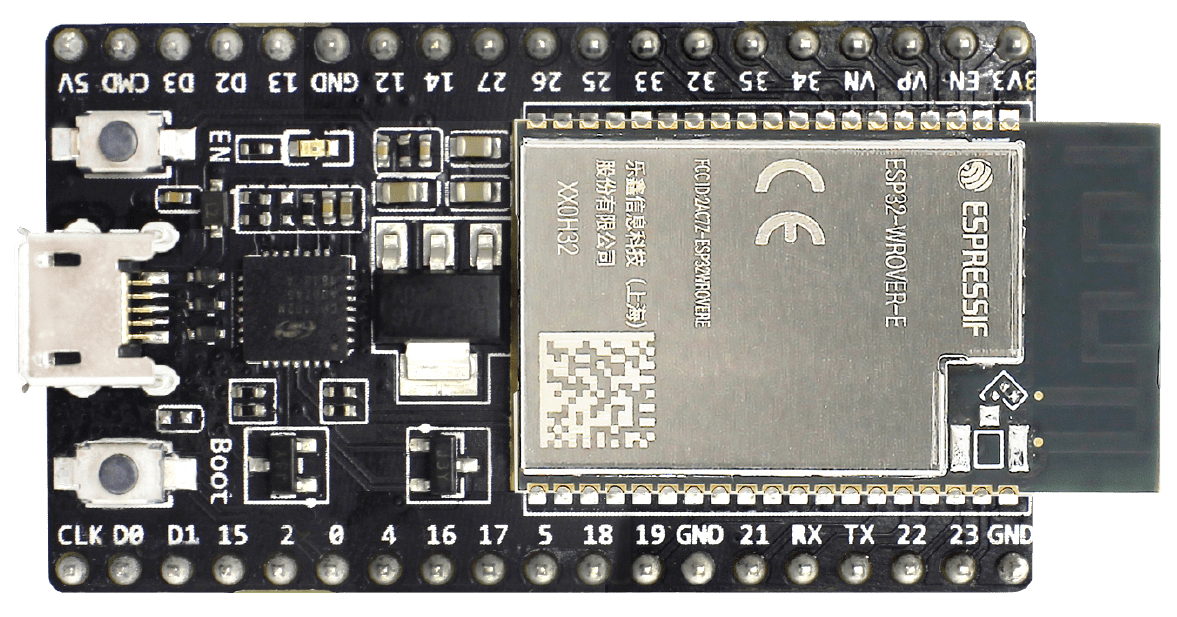
\includegraphics[scale=0.13]{figuras/esp323.png} 
    \legend{Fonte: Adaptado de \citeonline{espressifimg}.}
    \label{fig:esp32}
    \centering
\end{figure}

A versão escolhida para este projeto será o ESP32-CAM, onde além de possuir um 
\textit{chip} ESP32 integrado, nele também está incluso uma câmera, uma entrada para 
cartão SD e LED de alto brilho.

\subsection{PlatformIO}\label{sec:espacamento}

Uma forma para programar o ESP32 é utilizando o Arduino IDE. Um aplicativo de 
código aberto, escrito em C e C++, que permite a comunicação e gravação em \textit{chips} 
ATmega da família AVR. Entretanto, para gravar em \textit{chips} ESP32, basta ativar 
o utilitário Esptool.

Além do ambiente de desenvolvimento, outra vantagem é que o Arduino IDE 
possui inúmeras bibliotecas e documentação. Facilitando e assegurando o 
desenvolvimento de novos códigos, pois essas bibliotecas são constantemente 
testadas e atualizadas pela comunidade da plataforma Arduino.

\section{ESP-DL}\label{sec:formatacaoTexto}

ESP-DL é uma biblioteca de alto desempenho dedicada ao ESP32, ESP32-S2, 
ESP32-S3 e ESP32-C3, projetada para recursos de aprendizagem profunda. 

O \citeonline{espdl} oferece APIs para tarefas como inferência de redes 
neurais (NN), processamento de imagens, operações matemáticas e inclui 
alguns modelos de aprendizado profundo. Com essa biblioteca, você 
pode aproveitar os SoCs (System-on-Chip) da \textit{Espressif} de forma simples 
e ágil para implementar diversos tipo de aplicações.

\section{PROCESSAMENTO DE IMAGENS}\label{sec:processamento}

As técnicas de processamento de imagens começaram a surgir no final da década de 1960, 
para serem utilizadas no realce e restauração de imagens capturadas do espaço, 
como por exemplo, as imagens da missão Apollo. Logo em seguida essa tecnologia 
começou a ser empregada para processar imagens em diagnósticos médicos, e com 
o aumento de poder de processamento dos computadores, essas técnicas agora 
são empregadas nas mais diversas áreas de conhecimento \cite{gonzalez2010}.

Em processamento de imagens um conceito bastante utilizado é a binarização de
imagens, que consiste em duas classes distintas, o fundo e o objeto, esse processo 
serve para de certa forma separar ambas as classes.

Sendo assim, a forma mais simples de processamentos consiste na
bipartição do histograma, dando valores iguais a 0 (branco) aos pixels que estiverem
abaixo do valor de \textit{threshold} (T), e iguais a 255 (preto) aos pixels que estiverem 
acima desse valor. A \autoref{fig:escalacinza} mostra uma escala de tons 
de cinza, e a \autoref{fig:escalabinarizada} mostra essa mesma escala após passar 
por esse processamento, exemplificando o processo de binarização.

\begin{figure}[h!]
    \centering
    \caption{Escala de cinza}
    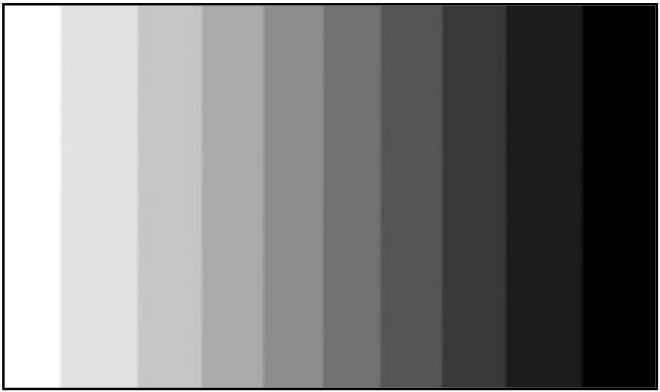
\includegraphics[scale=0.25]{figuras/escala_cinza.png} 
    \fonte{}%% Fonte
    \label{fig:escalacinza}
    \centering
\end{figure}

\begin{figure}[h!]
    \centering
    \caption{Escala de cinza binarizada}
    
\includegraphics[scale=0.25]{figuras/escala_binarizada.png} 
    \fonte{}%% Fonte
    \label{fig:escalabinarizada}
    \centering
\end{figure}

Especialmente durante o processo de reconhecimento de objetos. 
A segmentação é uma ferramenta indispensável para fins de análise e interpretação.

A segmentação de uma imagem é um procedimento importante no que tange
essas análises, uma vez que ela subdivide uma imagem em regiões que
posteriormente serão ou não tidas como de interesse, o que pode variar muito de
acordo com a aplicação \cite{gonzalez2010}.

Os principais algoritmos de segmentação se baseiam nas técnicas de
descontinuidade e similaridade, a abordagem de descontinuidade consiste em dividir
uma imagem com base nas mudanças bruscas mudanças de intensidade, como
ocorre nas bordas. Enquanto na técnica por similaridade a divisão da imagem
acontece por regiões que sejam semelhantes de acordo com um conjunto de critérios
preestabelecidos \cite{gonzalez2010}.

Por fim, uma outra técnica conhecida como esqueletização, 
consiste na representação de um conjunto de pontos no interior de um 
objeto de uma imagem. O esqueleto de uma região pode
ser definido pela transformada do eixo médio (MAT) do inglês (\textit{medial axis
transformation}). Nessa técnica são selecionados os elementos centrais de um objeto,
criando literalmente um esqueleto da imagem. MAT de uma região \textit{R} com uma borda
\textit{B} é definida como: para cada ponto \textit{p} contido na região, encontramos seu vizinho
mais próximo em \textit{B} (borda), e se houver mais de um vizinho então o ponto pertence
ao eixo médio, ou seja ao esqueleto \cite{gonzalez2010}.

O que pode ser visualizado com mais facilidade na \autoref{fig:esqueletizacao}:

\begin{figure}[h!]
    \centering
    \caption{Processo de esqueletização}
    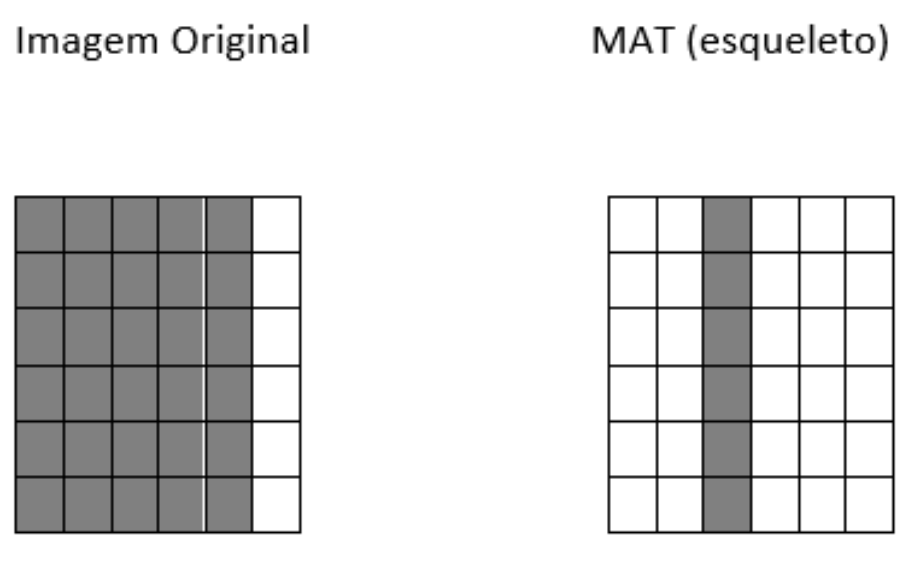
\includegraphics[scale=0.25]{figuras/esqueletizacao.png} 
    \fonte{}%% Fonte
    \label{fig:esqueletizacao}
    \centering
\end{figure}

\section{BIOMETRIA}\label{sec:biometria}

Com o avanço da tecnologia, hoje é possível realizar transações e pagamentos a 
partir de qualquer lugar, ou até mesmo, sem sair de casa, apenas com o uso de 
um dispositivo conectado a internet. Entretanto, também tornaram-se indispensáveis 
o uso de mecanismos de segurança, principalmente os que são capazes de identificar 
e comprovar quem realmente está utilizando esses serviços.

Por mais que existam outros processos de identificação, como por exemplo, cartões 
magnéticos, senhas, tags, etc., atualmente o processo considerado mais seguro é 
o baseado em biometria.

A biometria pode ser definida como o processo de identificação 
dos seres vivos. No intuito de distinguir os indivíduos, a partir de suas 
características únicas. É uma técnica que foi utilizada até mesmo pelos egípcios 
para o processo de identificação, baseando-se em características da
aparência dos indivíduos, como cor dos olhos e cicatrizes \cite{santos2007}.

\section{TIPOS DE BIOMETRIA}\label{sec:tiposBiometria}

De acordo com \citeonline{morais2010}, os principais tipos de biometria são:

\begin{itemize}
    \item Orelhas: Usa a anatomia da orelha para identificar indivíduos, abordagens 
    incomuns. Os pontos fortes são aceitabilidade e permanência; fraquezas, 
    singularidade e desempenho.

    \item Termograma da face e das mãos: O padrão de calor emitido pelo corpo 
    humano é uma característica de cada pessoa e pode ser captado por 
    infravermelho. Sistemas baseados em imagens termográficas não requerem 
    contato ou cooperação individual. No entanto, a captura de imagem continua 
    sendo um desafio em ambientes não controlados, pois é afetada por fontes de 
    calor que possivelmente podem estar próximas ao indivíduo. Seus pontos fortes 
    são a universalidade, a impostura e a singularidade.

    \item Impressão digital: recurso mais comumente usado em credenciais 
     automatizadas em grande escala.  Sua popularidade se deve em parte a 
     dispositivos de coleta de baixo custo e desempenho de processo razoável. 
     Embora a impressão digital não se modifique naturalmente ao longo dos anos, 
     ela é sensível aos fatores ambientais aos quais os indivíduos estão 
     submetidos, o que pode levar à sua alteração e deterioração. Trabalhadores 
     manuais, por exemplo, podem ver suas impressões digitais constantemente 
     alteradas devido a cortes profundos ou outros cortes em seus dedos.

    \item Íris: Formada durante o desenvolvimento fetal, estabiliza-se durante 
    os dois primeiros anos de vida. Sua textura é extremamente complexa e 
    fornece informações a serem utilizadas no reconhecimento facial. Tem um baixo grau 
    de impostura, pois é difícil até cirurgicamente alterar a textura da íris. 
    Seu ponto fraco está em sua capacidade de recuperação, requer equipamentos 
    caros e complexos, bem como cooperação individual.

    \item Voz: União de biometria comportamental e fisiológica. Ele não muda 
    em curtos períodos de tempo, mas é afetado por fatores como um simples frio, 
    estado emocional e ruído de fundo. Possui baixa exclusividade e não é 
    recomendado para identificação em larga escala. O ponto forte é a capacidade 
    de coleta e aceitabilidade, além do baixo custo dos coletores. Geralmente 
    indicado para verificação de identidade em conversas.
\end{itemize}

\section{RECONHECIMENTO FACIAL}\label{sec:reconhecimento}

Desde a infância, o ser humano adquire e desenvolve sua capacidade de reconhecer traços faciais, 
que é uma particularidade da visão e fundamental para relações sociais \cite{rouhani2019}.

Existem estudos sobre automatização do reconhecimento facial desde os anos 60. Os projetos iniciais nessa 
área dependiam do administrador encontrar manualmente as características faciais nas imagens, só 
então o sistema calculava as distâncias entre elas e comparava suas dimensões normalizadas com 
as referenciadas.

O processo de reconhecimento facial pode ser descrito a partir de uma imagem ou vídeo estático, 
identificando um ou múltiplos indivíduos a partir de um banco de dados de rostos previamente 
cadastrados. Assim, existem três abordagens conhecidas para reconhecimento:

\begin{itemize}
    \item Imagem a imagem: a amostra e a base de dados composta por imagens estáticas;

    \item Vídeo para vídeo: a amostra e o banco de dados que consiste em vídeos;

    \item Imagem para vídeo: o exemplo é um vídeo. O vídeo é comparado a um banco de 
    dados de imagens estáticas. Para esse caso, a biblioteca OpenCV possibilita,
     a partir da versão 2.4, o uso da classe FaceRecognizer para reconhecimento 
     facial. Os algoritmos atualmente disponíveis na biblioteca são: Fisherfaces 
     e Histogramas de Padrões Binários Locais (LBP).
\end{itemize}

Após a imagem ter sido lida e transformada em uma matriz da OpenCV, a mesma é
duplicada e redimensionada proporcionalmente para uma altura fixa. A imagem original 
é mantida para ser utilizada posteriormente. Em seguida a imagem é convertida para 
escalas de cinza e então equalizada para realçar o contraste e facilitar a detecção de faces.

A seguir, é feita a detecção das faces utilizando o classificador LBP
fornecido pela biblioteca OpenCV. Removendo o fundo ao redor da face, pois 
pode atrapalhar os algoritmos de reconhecimento.

As abordagens mais populares usadas no problema de reconhecimento facial são 
baseadas na localização e análise de atributos faciais como olhos, nariz e boca (\autoref{fig:haarcascate}), 
ou em análise global destes.

\begin{figure}[h!]
    \centering
    \caption{Reconhecimento baseado na localização dos olhos e nariz}
    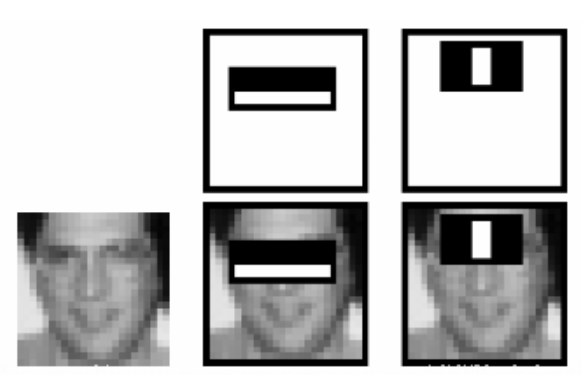
\includegraphics[scale=0.25]{figuras/haarcascate.png}
    \legend{Fonte: Adaptado de \citeonline{viola2004}.}
    \label{fig:haarcascate}
    \centering
\end{figure}

E com a comparação das informações extraídas com as informações
conhecidas, juntamente com uma pequena análise estatística, pode-se categorizar o
objeto e ainda determinar com precisão do que se trata \cite{gonzalez2010}.

\section{BIOMETRIA FACIAL PARA CONTROLE E ACESSO}\label{sec:biometriaFacial}

Os sistemas de identificação baseados em biometria são essencialmente sistemas de 
reconhecimento que, dadas informações biométricas, são capazes de distinguir padrões e 
classificá-los em diferentes classes ou categorias. \cite{morais2010}.

Ainda de acordo com o autor, algumas das principais características anatômicas, 
fisiológicas e comportamentais utilizadas em sistemas biométricos incluem 
impressão digital, impressão da mão, aparência facial, temperatura da face, 
retina, voz, assinatura, entre outras.

A biometria facial é o recurso biométrico mais utilizado por humanos para identificação 
pessoal. Embora usar a face para identificar conhecidos seja uma tarefa trivial para 
o ser humano, no entanto, é uma tarefa bastante complexa para computadores. Mesmo 
tendo um desempenho razoável em sistemas comerciais, um sistema biométrico facial 
impõem algumas restrições no fundo, como iluminação e o ângulo das imagens utilizadas.

Segundo \citeonline{cavalcanti2005}, alterações estéticas, como cabelo e barba, uso de
acessórios, como óculos e bonés, são fatores que aumentam as chances de falha no processo
de reconhecimento facial.

Para utilizar a face em sistemas biométricos é preciso seguir três
etapas fundamentais. São elas:

\begin{itemize}
    \item Detecção Facial: Responsável por definir e localizar uma ou mais
    faces;

    \item Extração de Características: Esta fase é responsável por remover o excesso de
    informações que rodeiam as faces detectadas, assim como selecionar as melhores
    características para serem utilizadas na próxima etapa;

    \item Reconhecimento Facial: Esta fase compara as características selecionadas pela fase
    anterior com outras previamente cadastradas em um banco de dados. Sendo
    responsável por encontrar um registro que se assemelhe ao que precisa ser
    identificado;

\end{itemize}%% Comente para remover este item

%% Capítulo
%% ATENÇÃO - veja com o seu orientador se você vai ter este capítulo e se este vai ter nome!
\chapter{Trabalhos Relacionados}
\label{cap:trabalhos:relacionados}

Apresente aqui os trabalhos similares ao seu trabalho ou que são importantes para o entendimento do seu trabalho...

%---------------------------------------------------%

%% Comente para remover este item

%% Capítulo
%\include{./capitulos/cap-proposta}%% Comente para remover este item

%% Capítulo
%%%% CAPÍTULO 3 - MATERIAL E MÉTODOS (PODE SER OUTRO TÍTULO DE ACORDO COM O TRABALHO REALIZADO)

\chapter{Metodologia}\label{cap:materialemetodos}

O trabalho será dividido em três etapas principais: o desenvolvimento do \textit{software}, 
do \textit{hardware}, e a execução dos testes. Sendo a primeira etapa 
destinada ao desenvolvimento do algoritmo de reconhecimento facial, utilizando os 
recursos da biblioteca OpenCV para o processamento de imagens.

O fluxograma da \autoref{fig:fluxoprog} mostra de maneira simplificada e intuitiva
como o sistema vai tratar as entradas dos sinais (imagens), até validar os resultados.

\begin{figure}[h!]
    \centering
    \caption{Fluxograma do \textit{firmware}}
    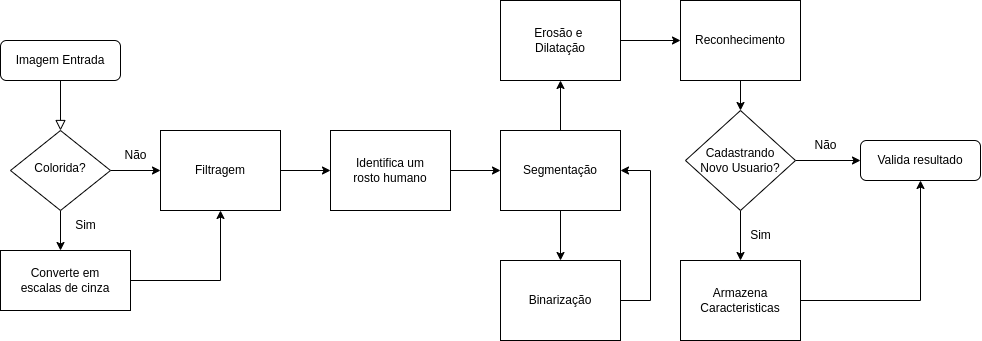
\includegraphics[scale=0.4]{figuras/fluxo_programa.png} 
    \fonte{}%% Fonte
    \label{fig:fluxoprog}
    \centering
\end{figure}

Porém para executar esse algoritmo, será necessário a utilização de um \textit{hardware} 
capaz de processá-lo, desta forma, a segunda etapa será responsável pela montagem 
do protótipo. No intuito de facilitar a compreensão do seu funcionamento, o diagrama da 
\autoref{fig:fluxohard} foi criado. Onde no protótipo serão utilizados módulos para alimentação, 
aquisição dos sinais e processamento, interface gráfica e por fim, um módulo para 
acionamento da fechadura.

\begin{figure}[h!]
    \centering
    \caption{Diagrama de blocos do \textit{hardware}}
    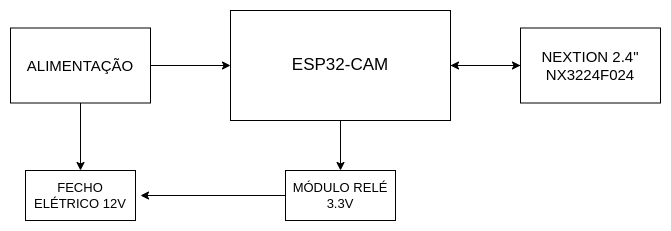
\includegraphics[scale=0.4]{figuras/fluxo_hardware.png} 
    \fonte{}%% Fonte
    \label{fig:fluxohard}
    \centering
\end{figure}

A terceira e última etapa será referente a validação do protótipo, desde testes, 
ajustes no algoritmo, até melhorias e atualização no \textit{hardware}. Nessa etapa será 
analisada a assertividade do código desenvolvido e também a sua viabilidade para
utilização no dia-a-dia.

\section{Computador de placa única}\label{sec:materiais}

O módulo principal do protótipo, será o ESP32-CAM (\autoref{fig:espcam}) da Espressif®. 
Este dispositivo apesar de ser simples e compacto é ideal para este projeto,  
pois além de possuir uma câmera integrada a sua placa, possui uma capacidade de 
execução em quase tempo real. Sendo este também, o responsável por 
processar, analisar e controlar os demais \textit{hardwares}. 

\begin{figure}[h!]
    \centering
    \caption{ESP32-CAM}
    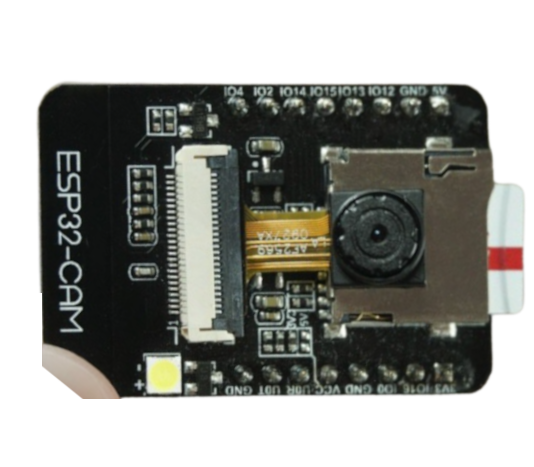
\includegraphics[scale=0.25]{figuras/esp32cam.png} 
    \legend{Fonte: Adaptado de \citeonline{espcamimg}.}
    \label{fig:espcam}
    \centering
\end{figure}

\section{Interface gráfica}\label{sec:materiais}

Para uma melhor interação do usuário com o protótipo, será utilizado o \textit{hardware} 
Nextion Intellignet (\autoref{fig:nextion}), \textit{display} capaz de fornecer uma interface de controle e visualização 
de forma simples e rápida. Além desses fatores, essa placa possui um editor visual 
com inúmeros componentes e recursos, desta forma, facilitando e reduzindo o tempo 
de programação.

\begin{figure}[h!]
    \centering
    \caption{Nextion Intellignet}
    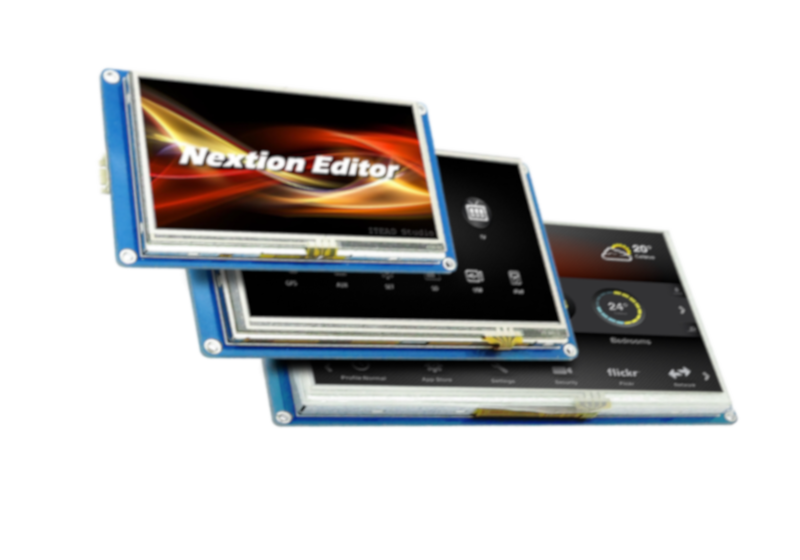
\includegraphics[scale=0.3]{figuras/nextion.png} 
    \legend{Fonte: Adaptado de \citeonline{nextionimg}.}
    \label{fig:nextion}
    \centering
\end{figure}

\section{Módulo de acionamento}\label{sec:materiais}

Os relés são adequados para acionar dispositivos eletrônicos como luzes, 
ventiladores, ar condicionado, etc. E atualmente são muito 
utilizados em sistemas de automação residencial e industrial, devido a 
facilidade em controlar cargas CA de média e alta tensão, a partir de 
circuitos CC de baixa tensão. Desta forma, o acionamento do protótipo 
será feito, por meio de um módulo relé (\autoref{fig:rele}).

\begin{figure}[h!]
    \centering
    \caption{Módulo Relé}
    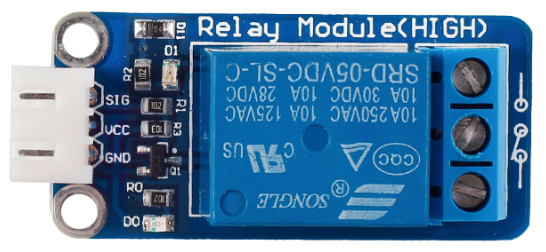
\includegraphics[scale=1]{figuras/rele.png} 
    \fonte{\citeonline{releimg}}%% Fonte \legend{Fonte: Adaptado de \citeonline{releimg}.}
    \label{fig:rele}
    \centering
\end{figure}

\section{Fechadura eletrônica}\label{sec:materiais}

O controle de acesso só será funcional se houver uma fechadura eletrônica 
integrada ao seu sistema. Desta forma, o protótipo utilizará o Fecho Elétrico (\autoref{fig:fecho}) 
da AGL. Este que é indicado para portas internas, seja de madeira ou metal, sendo 
acionado por uma tensão em 12v. Desta forma, se o usuário estiver cadastrado 
e o sistema validar suas credenciais, a trava elétrica será acionada e 
então o acesso será liberado.


\begin{figure}[h!]
    \centering
    \caption{Fecho Elétrico}
    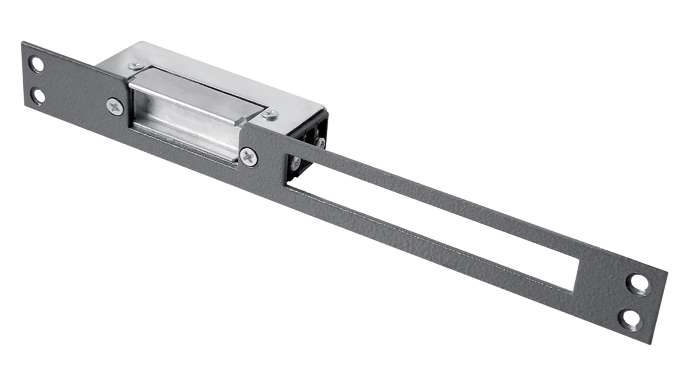
\includegraphics[scale=0.3]{figuras/fechoagl.png} 
    \fonte{\citeonline{fechaduraimg}}%%\legend{Fonte: Adaptado de \citeonline{fechaduraimg}.}
    \label{fig:fecho}
    \centering
\end{figure}%% Comente para remover este item

%% Capítulo
%%%% CAPÍTULO 4 - RESULTADOS E DISCUSSÃO

\chapter{Resultados}\label{cap:resultados}

Este capítulo apresenta o que foi obtido como resultado do trabalho, que, em princípio, é o sistema desenvolvido. Se não for um sistema, como, por exemplo, uma solução na área de redes, neste capítulo é reportada a solução proposta. Neste caso, a divisão do capítulo em seções é realizada, se necessária, de acordo com o trabalho.

O capítulo pode conter seções de acordo com o tipo de sistema e a necessidade de documentação mais extensa de determinados aspectos. Caso o trabalho se refira à comparação entre tecnologias ou dados obtidos como resultados do uso do sistema, além da descrição do sistema, há os dados obtidos com os testes e a discussão desses dados. Nesse caso haverá uma seção para os dados obtidos desses testes e as discussões.

\section{Escopo do sistema}\label{sec:escopoSistema}

Apresenta o escopo do sistema (contendo entre dois ou cinco parágrafos) de forma bastante sucinta, considerando aspectos técnicos e conceituais. O escopo define o que é o sistema, consistindo das funcionalidades e características que o sistema deve conter. É importante apresentar também o escopo negativo, ou seja, as funcionalidades e características que o sistema não irá conter. 
Exemplo:

O sistema XYZ deve gerenciar todos os processos de uma livraria virtual, desde a aquisição até a venda dos livros para o consumidor final. O acesso dos compradores e gerentes deve ser feito por meio de um site WEB, incluindo a possibilidade de acesso por outras tecnologias (ex. celular, tablet). Os clientes poderão fazem as compras pagando com cartão de crédito ou depósito bancário. Existem promoções eventuais pelas quais os livros podem ser comprados com desconto.

De início, a livraria vai trabalhar apenas com livros novos a serem adquiridos de editoras que tenham sistema automatizado de aquisição. Desta forma, o sistema a ser desenvolvido deve conectar-se aos sistemas das editoras para efetuar as compras.

O sistema deve calcular o custo de entrega baseado no peso dos livros e na distância do ponto de entrega. Eventualmente podem haver promoções do tipo “entrega gratuita” para determinadas localidades.

O sistema deve permitir a um gerente emitir relatórios de livros mais vendidos, e compradores mais assíduos, bem como sugerir compras para compradores baseadas em seus interesses anteriores.

\section{Modelagem do sistema}\label{sec:modelagemSistema}

A modelagem do sistema inclui os diagramas e as descrições textuais para representar o problema e a solução.

Sendo assim, primeiramente esse item deve apresentar diagramas utilizados para a modelagem de negócios (ex. diagramas de atividade e estado), se esses tenham sido necessários.
Em seguida esse item deve conter a descrição dos requisitos obtidos do usuário, contendo sua respectiva classificação (funcionais e não funcionais). Sugere-se o uso de um modelo formal sugerido por autores (ex. Wazlawick, Bezerra) para a apresentação dessa classificação.

Se utilizada orientação a objetos e a UML, nesta seção ainda são apresentados, por exemplo, os diagramas de casos de uso, com suas descrições suplementares, os diagramas de classe de análise (ou modelo conceitual), de sequência e/ou comunicação, diagrama de classes de projeto.

Nesta seção também estão os diagramas da modelagem de banco de dados, como entidade-relacionamento. Nesse item pode ser apresentada a descrição de cada uma das classes do modelo de classes apresentado acima, assim como a descrição das tabelas do banco de dados. Também podem estar documentados modelos e padronizações utilizados para a interface, diagramas de navegação, a representação da arquitetura do sistema e dos padrões de projeto utilizados.

\section{Apresentação do sistema}\label{sec:apresentacaoSistema}

Apresenta as funcionalidades e o uso de recursos tecnológicos do sistema por meio de suas telas, enfatizando a interação com o sistema. A apresentação do sistema é feita sob a forma de texto, com telas e definição de padrões que forem relevantes ao contexto do trabalho. As telas são tratadas como figuras, cópias (print screen) de relatórios ou consultas também são figuras.

A \autoref{fig:cadastroPaciente} exibe a tela de acesso ao Cadastro de Pacientes.

\begin{figure}[htpb]%% Ambiente figure
\caption{Tela de acesso ao Cadastro de Pacientes.}%% Legenda
\label{fig:cadastroPaciente}%% Rótulo
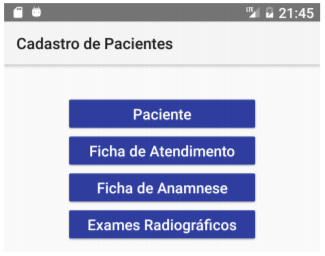
\includegraphics[scale=0.8]{cadastro-paciente}%% Dimensões e localização
\fonte{}%% Fonte
\end{figure}

\section{Implementação do sistema}\label{sec:implementacaoSistema}

Nesta seção é documentada a implementação do sistema com partes relevantes ou exemplos de código, rotinas, funções. Inclui, ainda, a descrição técnica do uso de recursos (componentes, bibliotecas, etc.) da linguagem. Ressalta-se que cada orientador avaliará juntamente com seu orientado o que poderá ser descrito nesta seção. Isso sem que sejam revelados detalhes do sistema que possam comprometer seu uso comercial ou científico ou que a descrição fique muito sucinta ou superficial.

Em materiais e método estão quais os recursos utilizados, neste capítulo é reportado como esses recursos foram utilizados para resolver o problema.

Sugere-se colocar listagens curtas de código, enfatizando aspectos específicos das tecnologias utilizadas ou da implementação. Sugere-se, ainda, que o código não seja apresentado sob a forma de print screen, e sim copiado e colado no texto, mantendo, se possível, a formatação. Todas as listagens de código devem ser devidamente explicadas. A explicação deve ser técnica, fundamentada em aspectos conceituais e boas práticas de programação.

Enfatizar os diferenciais do sistema: procedimentos armazenados, consultas SQL, uso de componentes, uso de padrões de projeto, a forma de uso dos recursos da linguagem. Esses diferenciais são no sentido de explicitar as vantagens, desvantagens, dificuldades e facilidades que esses recursos impetraram no desenvolvimento do sistema em termos técnicos. Esses diferenciais servirão para avaliar pela utilização ou não desses recursos, pelo menos para sistemas iguais ou semelhantes ao reportado no trabalho.

Reportar a forma como o sistema foi verificado e validado. No sentido de verificar se os requisitos definidos para o mesmo foram atendidos. Os testes podem ser realizados pelo professor orientador, pelos professores que compõem a banca, por pessoas que serviram de base para as informações para o sistema e etc. Os testes podem ser realizados com base em um plano de testes elaborado juntamente com a análise e projeto do sistema. Para validar a implementação podem ser desenvolvidas rotinas de teste unitário.

Se houver implantação do sistema, mesmo que seja para teste, reportar a forma como isso foi feito, a geração de instaladores, os problemas com ambiente e sistema operacional, incluindo banco de dados e outros. Deixar explícito o procedimento para instalar e usar o sistema.

Quando for necessário, citar no texto do trabalho nomes de campos, tabelas ou rotinas específicas utilizadas na implementação de um software, utilizar a fonte courier new para destacar esses nomes.

Um exemplo de listagem de código fonte pode ser observado na \autoref{codigo:classeFoo}, que representa a classe Aluno.

\begin{sourcecode}[htb]
\caption{\label{codigo:classeFoo}Classe Aluno}
\begin{lstlisting}[frame=single, language=Java]
@Entity
public class Foo {
 
    @Id
    @GeneratedValue(strategy = GenerationType.IDENTITY)
    private Long id;
 
    private String nome;
    
    private Integer ra;
     
    // constructor, getters and setters
}
\end{lstlisting}
\fonte{}
\end{sourcecode}

\section{Discussões (opcional)}\label{sec:discussoes} 

O trabalho contém esta seção quando considerado que há resultados (em termos de dados) e discussões relevantes ou suficientes para justificar uma seção. Se existentes e não justificarem uma seção, eles podem estar na seção que relata a implementação do sistema.

Nesta seção estão os resultados obtidos da realização de testes quantitativos e qualitativos, independentemente da quantidade, tipo e volume de testes realizados. Os resultados dos testes são discutidos tendo como base o referencial teórico e os objetivos pretendidos com o trabalho. Esses testes podem resultar de implantação e testes de uso do sistema. 
%% Comente para remover este item

%% Capítulo - esse capítulo contém exemplos para melhor uso do modelo Latex
%% Na versão final do TCC esse capítulo deve ser removido utilizando o sinal %
%%%%% CAPÍTULO - EXEMPLO
%%
%% Capítulo de informações e exemplos de utilização deste modelo.

%% Título e rótulo de capítulo (rótulos não devem conter caracteres especiais, acentuados ou cedilha)
\chapter{Informações e Exemplos de Utilização deste Modelo}\label{cap:exemplo}

Devido à necessidade de padronização em trabalhos acadêmicos (teses, dissertações, trabalhos de conclusão de curso, etc.), são utilizadas neste documento algumas regras básicas para estruturação e formatação.

O presente documento/\textit{template} foi produzido em parceria entre a \gls{utfpr} de Pato Branco e a \gls{utfpr} de Campo Mourão. Assim, derivado do \gls{utfprpbtex}\index{UTFPRPBTeX@\utfprpbtex} e de alterações implementadas pela UTFPR de Campo Mourão, surge o \utfprtex, como um proposta de um modelo \latex que pode ser utilizado por qualquer campus da \gls{utfpr} para elaboração de trabalhos acadêmicos segundo as normas definidas pela \gls{abnt}\index{ABNT}. Este modelo foi desenvolvido em linguagem de editoração \gls{tex}\index{TeX@\TeX}/\gls{latex}\index{LaTeX@\latex} com base no modelo \gls{abntex2}\index{abnTeX2@\abnTeX} \cite{abnTeX2:2013}, que atende os requisitos das normas da ABNT para elaboração de documentos técnicos e científicos brasileiros.

Os principais arquivos do modelo são: 
\begin{itemize}
    \item \texttt{main.tex} - é o arquivo principal que relaciona todos os outros arquivos, neste você pode remover ou adicionar elementos textuais (capítulos, etc);
    \item \texttt{configuracoes.tex} - contém os pacotes a serem utilizados pelo ambiente, bem como a criação de comandos do \latex;
    \item \texttt{variaveis.tex} - contém variáveis, como nome do autor, orientador, título, banca e que devem ser alterados para atender cada trabalho;
    \item \texttt{main.bib} - contém as referências bibliográficas;
    \item \texttt{readme.md} - são informações a respeito do template \latex;
    \item \texttt{utfpr.cls} - mantém a formatação do texto - \textbf{não altere esse arquivo a menos que você saiba o que está fazendo}.
\end{itemize}

Além dos arquivos, o \textit{template} contém diretórios/pastas, para ajudar a organizar o trabalho, sendo essas:
\begin{itemize}%% Lista de itens
\item \texttt{PreTexto} - contém arquivos, com nomes auto descritivos, que representam elementos pré textuais como:  resumo, abstract, agradecimentos, siglas, epigrafe, etc;
\item \texttt{capitulos} -  contém arquivos, com nomes auto descritivos, que representam os capítulos do texto, como por exemplo: introdução, metodologia, conclusão, etc. Para adicionar ou remover um capítulo é necessário alterar o arquivo \texttt{main.tex} - ver exemplos no próprio arquivo;
\item \texttt{figuras}  - contém as figuras/imagens utilizadas no texto;
\item \texttt{PosTexto} - contém elementos pós textuais como: anexo, apêndice, etc.
\end{itemize}

A codificação de caracteres em todos os arquivos é \texttt{UTF8}, tanto no modelo \gls{abntex2}\index{abnTeX2@\abnTeX} quanto no modelo \gls{utfprpbtex}\index{UTFPRPBTeX@\utfprtex}. Portanto, é necessário que seja utilizada a mesma codificação nos documentos a serem desenvolvidos, inclusive nos arquivos de base bibliográfica. Diversos editores de arquivos fonte do \gls{latex}\index{LaTeX@\latex} são capazes de manipular e/ou converter entre diferentes codificações, por exemplo, o ``Texmaker\index{Texmaker}'' (disponível em \url{http://www.xm1math.net/texmaker/}). 
%Recomenda-se, sempre que for manipular e/ou substituir um dos arquivos constituintes deste modelo, manter uma cópia do original num local seguro e/ou renomear esta cópia do original para que possa ser utilizada como um exemplo no desenvolvimento do seu próprio arquivo. Por exemplo, quando for criar o seu ``Capítulo 1'', fazer uma cópia do arquivo original \texttt{capitulo1.tex}, renomeando-o para \texttt{capitulo1.original.tex}, por exemplo, e realizar as alterações e/ou modificações no arquivo \texttt{capitulo1.tex}.

Este capítulo\label{errata:capitulo} de exemplo tem por finalidade a definição e a apresentação de alguns comandos do \gls{latex}\index{LaTeX@\latex} e/ou dos modelos \gls{abntex2}\index{abnTeX2@\abnTeX} e \gls{utfprpbtex}\index{UTFPRPBTeX@\utfprtex}. O presente documento não se constitui um manual, tampouco uma apostila de \gls{latex}\index{LaTeX@\latex}, visto que existe uma grande quantidade de material de referência disponível na Internet, como por exemplo em \url{http://en.wikibooks.org/wiki/LaTeX}.

Os capítulos devem conter uma introdução e um fecho. A introdução fornece ao leitor uma breve descrição do que será tratado no capítulo, enquanto o fecho apresenta comentários finais sobre o que foi desenvolvido no capítulo. Os capítulos podem ser divididos em seções\label{errata:secao}. Esta divisão deve ser lógica (temática) e não física (por tamanho). O número ideal de seções é impossível de se precisar. Entretanto, um capítulo com uma única seção, possivelmente, deverá ser agregado ao capítulo anterior ou posterior. Um capítulo com quinze seções, possivelmente, deverá ser subdividido em dois capítulos. Capítulos, seções e subseções\label{errata:subsecao} devem ser rotulados para que possam ser referenciados em qualquer parte do texto. Exemplo: O \autoref{cap:exemplo} é gerado, rotulado e referenciado pelos comandos \verb|\chapter{Informações e...}|, \verb|\label{cap:exemplo}| e \verb|\autoref{cap:exemplo}|, respectivamente.

%% Título e rótulo de seção (rótulos não devem conter caracteres especiais, acentuados ou cedilha)
\section{Título da seção secundária}\label{sec:secsec}

Seções secundárias são divisões do conteúdo das seções primárias. A \autoref{sec:secsec} é gerada, rotulada e referenciada pelos comandos \verb|\section{Título da Seção Secundária}|, \verb|\label{sec:secsec}| e \verb|\autoref{sec:secsec}|, respectivamente.

%% Título e rótulo de seção (rótulos não devem conter caracteres especiais, acentuados ou cedilha)
\subsection{Título da seção terciária}\label{ssec:secterc}

Seções terciárias são divisões do conteúdo de seções secundárias. A \autoref{ssec:secterc} é gerada, rotulada e referenciada pelos comandos \verb|\subsection{Título da Seção Terciária}|, \verb|\label{ssec:secterc}| e \verb|\autoref{ssec:secterc}|, respectivamente.

%% Título e rótulo de seção (rótulos não devem conter caracteres especiais, acentuados ou cedilha)
\subsubsection{Título da seção quartenária}\label{sssec:secquart}

Seções quartenárias são divisões do conteúdo de seções terciárias. A \autoref{sssec:secquart} é gerada, rotulada e referenciada pelos comandos \verb|\subsubsection{Título da seção quartenária}|, \verb|\label{sssec:secquart}| e \verb|\autoref{sssec:secquart}|, respectivamente.

%% Título e rótulo de seção (rótulos não devem conter caracteres especiais, acentuados ou cedilha)
\section{Exemplo de título de seção secundária com um texto muito longo que pode ocupar mais de uma linha}\label{sec:sectitulolongo}

A \autoref{sec:sectitulolongo} é um exemplo de título de seção secundária com texto muito longo, formatado automaticamente de acordo com \citeonline[subseções 5.2.2 a 5.2.4]{NBR14724:2011} e \citeonline[subseções 3.1 a 3.8]{NBR6024:2012}. Segundo as normas, o título de seção deve estar alinhado à esquerda e a segunda e demais linhas devem iniciar logo abaixo da primeira palavra da primeira linha.

%% Título e rótulo de seção (rótulos não devem conter caracteres especiais, acentuados ou cedilha)
\section{Elementos pré-textuais}\label{sec:elempretext}

Alguns elementos pré-textuais do presente documento são gerados automaticamente pelo \gls{utfprpbtex}\index{UTFPRPBTeX@\utfprtex}. Para adicionar e/ou alterar as informações apresentadas na capa, na folha de rosto %, na ficha catalográfica 
e na folha de aprovação deve-se editar o arquivo \texttt{variaveis.tex}. %Os dados informados neste arquivo também são utilizados para gerar a referência do trabalho na errata, no resumo e no \textit{abstract}.

Para adicionar e/ou alterar o texto da errata, da dedicatória, dos agradecimentos, da epígrafe, do resumo e do \textit{abstract} deve-se editar seus respectivos arquivos presentes no diretório ``PreTexto'': \texttt{errata.tex}, \texttt{dedicatoria.tex}, \texttt{agradecimentos.tex}, \texttt{epigrafe.tex}, \texttt{resumo.tex} e \texttt{abstract.tex}.

As listas de algoritmos, de ilustrações e de tabelas são geradas automaticamente pelo \gls{utfprpbtex}\index{UTFPRPBTeX@\utfprtex}. Os itens destas listas são gerados a medida que forem sendo inseridos no texto do documento. 

A lista de abreviaturas, siglas e acrônimos pode ser gerada automaticamente por meio do arquivo \texttt{entradas-acronimos.tex}, utilizando o pacote \texttt{glossaries}\footnote{Detalhes sobre comandos para geração de abreviaturas, siglas e acrônimos utilizando o pacote \texttt{glossaries} são apresentadas na \autoref{sec:acronimos}.}, ou por meio da edição do arquivo \texttt{lista-acronimos.tex}. A lista de símbolos pode ser gerada automaticamente utilizando o pacote \texttt{nomencl}\footnote{Detalhes sobre comandos para geração de símbolos utilizando o pacote \texttt{nomencl} são apresentadas na \autoref{sec:simbolos}.} ou mediante a edição do arquivo \texttt{lista-simbolos.tex}. Os arquivos citados estão no diretório ``PreTexto''. O sumário é o último elemento pré-textual e também é gerado automaticamente pelo \gls{utfprpbtex}\index{UTFPRPBTeX@\utfprtex}.

%% Título e rótulo de seção (rótulos não devem conter caracteres especiais, acentuados ou cedilha)
\section{Regras gerais de apresentação}\label{sec:regrasgerais}

As regras gerais de apresentação, definidas na sequência, já estão predefinidas no modelo \gls{utfprpbtex}\index{UTFPRPBTeX@\utfprtex}. Algumas destas regras podem ser alteradas, por comandos apropriados do \gls{latex}\index{LaTeX@\latex}, do \gls{abntex2}\index{abnTeX2@\abnTeX} ou do \gls{utfprpbtex}\index{UTFPRPBTeX@\utfprtex}, no preâmbulo do arquivo principal \texttt{configuracoes.tex} ou em outras partes do documento, por exemplo, nos capítulos.

\begin{itemize}%% Lista de itens
\item Configuração das margens: deve-se usar margens superior e esquerda de \SI{3}{cm}; e margens inferior e direita de \SI{2}{cm}; em papel formato A4 ($\SI{21}{cm} \times \SI{29,7}{cm}$);
\item Recomenda-se o uso de fonte tipo Arial ou Times New Roman, tamanho 12 para o texto e tamanho 10 para citações de mais de três linhas, notas de rodapé e legendas dos algoritmos, ilustrações e tabelas;
\item O parágrafo deve aparecer com recuo na primeira linha de \SI{1,5}{cm}, justificado, sem espaçamento anterior ou posterior;
%\item Os elementos como: o resumo, as notas, as referências, as legendas das ilustrações e tabelas, a natureza do trabalho, o objetivo, o nome da instituição a que é submetida e a área de concentração devem ser digitados em espaço simples.
\item A numeração progressiva para as seções do texto deve ser adotada para evidenciar a sistematização do conteúdo do trabalho;
\item Para os títulos das seções não se utilizam pontos, hífen, travessão, ou qualquer sinal após o indicativo de seção ou de título;
\item Para as seções primárias: utiliza-se negrito e caixa alta;
\item Para as seções secundárias: título em negrito, iniciado em letra maiúscula e demais letras minúsculas;
\item Para as seções terciárias: somente a primeira letra do título da seção em
maiúscula;
\item Para as seções quaternárias: título da seção sublinhado, com inicial em letra maiúscula e demais letras minúsculas.
\item No sumário, os títulos das seções devem aparecer exatamente iguais ao que estão contidos no trabalho.
\end{itemize}

\caixa{Atenção}{No \latex é necessário apenas manter os títulos apenas com a primeira letra maiúscula e o restante em minúsculo, o retante é controlado pelo \latex, então não é necessário se preocupar com a formatação!}

Recomenda-se evitar, sempre que possível, o uso dos seguintes recursos (ou enfeites) no documento:

\begin{itemize}%% Lista de itens
\item \textbf{o uso de negrito;}
\item \textit{o uso de itálico (exceto em palavras em outra língua);}
\item \texttt{texto em diferente fonte como máquina de escrever;}
\item \underline{o uso de texto sublinhado;}
\item o uso excessivo de\footnote{Notas de rodapé.}.
\end{itemize}

\noindent Lembre-se: um texto ``limpo'' é mais agradável de ler que um texto ``enfeitado''.

%% Título e rótulo de seção (rótulos não devem conter caracteres especiais, acentuados ou cedilha)
\subsection{Espaçamento}\label{sec:espacamento}

\begin{itemize}%% Lista de itens
%\item O resumo, o \textit{abstract}, as notas, as referências, as legendas das ilustrações e tabelas e a natureza do trabalho devem ser digitadas em espaço simples.
\item Todo o texto deve ser formatado com espaço entre linhas de um fator de 1,5 (sem espaçamento antes/depois).
\item As citações com mais de três linhas devem ser em espaço simples e com recuo de \SI{4}{cm} da margem esquerda.
\item As referências, ao final do trabalho, devem ser separadas entre si por um espaços simples, e na mesma referência o espaço é simples.
%\item Os títulos das seções secundárias devem ser separados do texto que os precede por dois espaços entre linhas de um fator de 1,5.
\item As seções primárias devem iniciar em páginas distintas.
\end{itemize}

O recuo na primeira linha, espaço entre a margem e o início do parágrafo, pode ser redefinido definido pelo comando:

\begin{SingleSpacing}%% Ambiente SingleSpacing
\begin{verbatim}
\setlength{\parindent}{1.5cm}
\end{verbatim}
\end{SingleSpacing}

O espaçamento entre um parágrafo e outro\index{espaçamento!entre os parágrafos} pode ser redefinido pelo comando:

\begin{SingleSpacing}%% Ambiente SingleSpacing
\begin{verbatim}
\setlength{\parskip}{0mm} %% Tente também \onelineskip
\end{verbatim}
\end{SingleSpacing}

O controle do espaçamento entre linhas\index{espaçamento!entre as linhas} pode ser redefinido pelo comando:

\begin{SingleSpacing}%% Ambiente SingleSpacing
\begin{verbatim}
\OnehalfSpacing %% Espaçamento um e meio (padrão)
\DoubleSpacing  %% Espaçamento duplo
\SingleSpacing  %% Espaçamento simples
\end{verbatim}
\end{SingleSpacing}

Para isso, também estão disponíveis os ambientes:

\begin{SingleSpacing}%% Ambiente SingleSpacing
\begin{verbatim}
\begin{SingleSpacing} ...     \end{SingleSpacing}
\begin{Spacing}{<factor>} ... \end{Spacing}
\begin{OnehalfSpacing} ...    \end{OnehalfSpacing}
\begin{OnehalfSpacing*} ...   \end{OnehalfSpacing*}
\begin{DoubleSpacing} ...     \end{DoubleSpacing}
\begin{DoubleSpacing*} ...    \end{DoubleSpacing*}
\end{verbatim}
\end{SingleSpacing}

Para mais informações, consulte \citeonline[p. 47-52 e 135]{Wilson2010}.

%% Título e rótulo de seção (rótulos não devem conter caracteres especiais, acentuados ou cedilha)
\section{Enumerações: alíneas e subalíneas}\label{sec:enumeracoes}\index{alíneas}\index{subalíneas}

Quando for necessário enumerar os diversos assuntos de uma seção que não possua título, esta deve ser subdividida em alíneas\index{alíneas} \cite[subseção 4.2]{NBR6024:2012}:

\begin{alineas}%% Ambiente alineas
\item os diversos assuntos que não possuam título próprio, dentro de uma mesma seção, devem ser subdivididos em alíneas\index{alíneas};
\item o texto que antecede as alíneas\index{alíneas} termina em dois pontos;
\item as alíneas\index{alíneas} devem ser indicadas alfabeticamente, em letra minúscula, seguida de parêntese. Utilizam-se letras dobradas, quando esgotadas as letras do alfabeto;
\item as letras indicativas das alíneas\index{alíneas} devem apresentar recuo em relação à margem esquerda;
\item o texto da alínea deve começar por letra minúscula e terminar em ponto-e-vírgula, exceto a última alínea que termina em ponto final;
\item o texto da alínea deve terminar em dois pontos, se houver subalínea;
\item a segunda e as seguintes linhas do texto da alínea começa sob a primeira letra do texto da própria alínea;
\item subalíneas\index{subalíneas} \cite[subseção 4.3]{NBR6024:2012} devem ser conforme as alíneas\index{alíneas} a seguir:
\begin{alineas}%% Ambiente alineas
\item as subalíneas\index{subalíneas} devem começar por travessão seguido de espaço;
\item as subalíneas\index{subalíneas} devem apresentar recuo em relação à alínea;
\item o texto da subalínea deve começar por letra minúscula e terminar em ponto-e-vírgula. A última subalínea deve terminar em ponto final, se não houver alínea subsequente;
\item a segunda e as seguintes linhas do texto da subalínea começam sob a primeira letra do texto da própria subalínea.
\end{alineas}
\item no \gls{abntex2}\index{abnTeX2@\abnTeX} estão disponíveis os ambientes \texttt{incisos} e \texttt{subalineas}, que em suma são o mesmo que se criar outro nível de \texttt{alineas}, como nos exemplos à seguir:
\begin{incisos}%% Ambiente incisos
\item \textit{um novo inciso em itálico}\index{incisos}.
\end{incisos}
\item Alínea em \textbf{negrito}:
\begin{subalineas}%% Ambiente subalineas
\item \textit{uma subalínea em itálico};
\item \underline{\textit{uma subalínea em itálico e sublinhado}}.
\end{subalineas}
\item última alínea com \emph{ênfase}.
\end{alineas}

%% Título e rótulo de seção (rótulos não devem conter caracteres especiais, acentuados ou cedilha)
\section{Citações}\label{sec:citacoes}

O \gls{utfprpbtex}\index{UTFPRPBTeX@\utfprtex} está configurado para produzir as citações no texto no estilo alfabético (autor-ano), segundo as normas \gls{abnt}\index{ABNT}, por meio dos comandos do \gls{abntex2}\index{abnTeX2@\abnTeX} \cite{abnTeX2:2013Cite,abnTeX2:2013CiteAlf}. A lista dos principais comandos são apresentadas a seguir:

\begin{itemize}%% Lista de itens
\item \verb|\cite{rótulo}| -- para gerar citação implícita. Por exemplo, a citação ``\ldots\ \cite{Thompson2001}\ldots'' é gerada pelo comando \verb|\cite{Thompson2001}| ou pelo atalho \verb|\citep{Thompson2001}|, definido em \texttt{utfprpb.tex}.
\item \verb|\citeonline{rótulo}| -- para gerar citação explícita. Por exemplo a citação ``\ldots\ conforme proposto por \citeonline{Thompson2001}\ldots'' é gerada pelo comando \verb|\citeonline{Thompson2001}| ou pelo atalho \verb|\citet{Thompson2001}|, definido em \texttt{utfprpb.tex}.
\item \verb|(\citeauthor{rótulo})| -- para gerar citação implícita somente do autor. Por exemplo, a citação ``\ldots\ (\citeauthor{Thompson2001})\ldots'' é gerada pelo comando \verb|(\citeauthor{Thompson2001})| ou pelo atalho \verb|\citepa{Thompson2001}|, definido em \texttt{utfprpb.tex}.
\item \verb|\citeauthoronline{rótulo}| -- para gerar citação explícita somente do autor. Por exemplo, a citação ``\ldots\ conforme a relação de \citeauthoronline{Thompson2001}\ldots'' é gerada pelo comando \verb|\citeauthoronline{Thompson2001}| ou pelo atalho \verb|\citeta{Thompson2001}|, definido em \texttt{utfprpb.tex}.
\item \verb|(\citeyear{rótulo})| -- para gerar citação implícita somente do ano. Por exemplo, a citação ``\ldots\ (\citeyear{Thompson2001})\ldots'' é gerada pelo comando \verb|(\citeyear{Thompson2001})| ou pelo atalho \verb|\citepy{Thompson2001}|, definido em \texttt{utfprpb.tex}.
\item \verb|\citeyear{rótulo}| -- para gerar citação explícita somente do ano. Por exemplo, a citação ``\ldots\ no ano de \citeyear{Thompson2001}\ldots'' é gerada pelo comando \verb|\citeyear{Thompson2001}| ou pelo atalho \verb|\citety{Thompson2001}|, definido em \texttt{utfprpb.tex}.
\end{itemize}

Informações sobre a utilização dos comandos listados acima e os demais comandos para geração de referências, utilizados pelo \gls{abntex2}\index{abnTeX2@\abnTeX}, podem ser encontradas em \citeonline{abnTeX2:2013Cite,abnTeX2:2013CiteAlf}, disponíveis em \url{http://www.abntex.net.br/}.

\gls{latex}\index{LaTeX@\latex} utiliza um arquivo externo (em separado) para o banco de dados das referências citadas no texto. Este arquivo é compilado pelo \gls{bibtex}\index{BibTeX@Bib\TeX} e deve possuir a extensão \texttt{bib}, como nos arquivos \texttt{referencias.bib} e \texttt{referencias-modelos.bib} presentes no diretório ``PosTexto'', utilizados neste documento. O arquivo \texttt{referencias-modelos.bib} apresenta exemplos dos seguintes estilos de referência aceitos pelo \gls{bibtex}\index{BibTeX@Bib\TeX}:

\begin{itemize}%% Lista de itens
\item anais de simpósios \citep{Alt1995,Pirmez2002};
\item artigos em anais de simpósios \citep{Faina2001};
\item artigos em coletâneas de artigos \citep{Pinto2000};
\item artigos em revistas \citep{Guimaraes2003};
\item capítulos de livros \citep{Santos2000};
\item livretos \citep{Thompson2001};
\item livros \citep{Pedrycz1998};
\item manuais técnicos \citep{IONA1999};
\item miscelânea \citep{Cruz2003};
\item páginas na Internet \cite[acessado em 1 de janeiro de 2004]{Larsson2003} (utilizar a data do último acesso à página);
\item relatórios técnicos \citep{OMG2000};
\item teses de mestrado \citep{SantosFilho2003};
\item teses de doutorado \citep{Faina2000};
\item trabalhos não publicados \citep{Sichman2002}.
\end{itemize}

Existem alguns programas para gerenciamento de banco de dados de referências bibliográficas (arquivos \texttt{bib}) do \gls{bibtex}\index{BibTeX@Bib\TeX}. O ``JabRef'' é um exemplo destes programas e está disponível em: \url{http://jabref.sourceforge.net/}.

%% Título e rótulo de seção (rótulos não devem conter caracteres especiais, acentuados ou cedilha)
\subsection{Citações Diretas}\label{sec:citacoesdiretas}\index{citações!diretas}

O ambiente \texttt{citacao} permite a inclusão de citações diretas que ocupam mais de três linhas:

\begin{citacao}%% Ambiente citacao
As citações diretas no texto, que ocupam mais de três linhas, devem ser destacadas com recuo de \SI{4}{cm} da margem esquerda, com letra menor que a do texto utilizado e sem as aspas. No caso de documentos datilografados, deve-se observar apenas o recuo \cite[subseção 5.3]{NBR10520:2002}.
\end{citacao}

\noindent Esta citação direta com mais de três linhas foi gerada da seguinte forma:

\begin{SingleSpacing}%% Ambiente SingleSpacing
\begin{verbatim}
\begin{citacao}
As citações diretas no texto, com mais de três linhas,...
... observar apenas o recuo \cite[subseção 5.3]{NBR10520:2002}.
\end{citacao}
\end{verbatim}
\end{SingleSpacing}

O ambiente \texttt{citacao} pode receber como parâmetro opcional um nome de idioma previamente carregado nas opções da classe (definido no preâmbulo do arquivo \texttt{utfprpb.tex}). Neste caso, o texto da citação é automaticamente escrito em itálico e a hifenização é ajustada para o idioma selecionado na opção do ambiente. Por exemplo:

\begin{SingleSpacing}%% Ambiente SingleSpacing
\begin{verbatim}
\begin{citacao}[english]
Text in English language in italic with correct hyphenation.
\end{citacao}
\end{verbatim}
\end{SingleSpacing}

\noindent Tem como resultado:

\begin{citacao}[english]%% Ambiente citacao
Text in English language in italic with correct hyphenation.
\end{citacao}

Citações simples\index{citações!simples}, com até três linhas, devem ser incluídas com aspas. Observe que em \gls{latex}\index{LaTeX@\latex} as aspas iniciais são diferentes das finais: ``Amor é fogo que arde sem se ver''.

%% Título e rótulo de seção (rótulos não devem conter caracteres especiais, acentuados ou cedilha)
\section{Equações}\label{sec:equacoes}

\gls{latex}\index{LaTeX@\latex} é insuperável no processamento de equações. Equações simples como $y = a x^2 + b x + c$ podem ser adicionadas ao longo do texto ou em uma linha própria:
%
\[%% Ambiente displaymath
y = a x^2 + b x + c
\]

Equações complexas como:
%
\begin{equation}%% Ambiente equation
\label{eq:equation1}%% Rótulo
\begin{array}{lcl}%% Ambiente array
p \left(\gamma\right)
& = &
\frac{1}{2}
\sqrt{\frac{M}{\gamma \bar{\gamma}_b}}
\frac{1}{\prod_{i = 1}^M \sqrt{\tilde{\gamma}_i}}
\int_0^{\sqrt{M \delta}}
\int_0^{\sqrt{M \delta} - r_M} \cdots
\int_0^{\sqrt{M \delta} - \sum_{i = 3}^M r_i} \\[0.5\linha]
& &
p \left(%
\frac{\sqrt{M \delta} - \sum_{i = 2}^M r_i}{\sqrt{\tilde{\gamma}_1}},
\frac{r_2}{\sqrt{\tilde{\gamma}_2}}, \ldots,
\frac{r_M}{\sqrt{\tilde{\gamma}_M}}
\right) \, \der r_2 \cdots \der r_{M - 1} \, \der r_M
\end{array}
\end{equation}

\noindent ou
%
\begin{equation}%% Ambiente equation
\label{eq:equation2}%% Rótulo
T \left(r\right) =
\frac{1}{f_m}
\left(%
\frac{\pi}{2} \sum_{i = 1}^M {\tilde{r}_i^2 \dot{\varsigma}_i^2}
\right)^{-1/2}
\frac{%
\begin{array}{ll}%% Ambiente array
\int_0^{\rho \sqrt{M}}
\int_0^{\rho \sqrt{M} - r_M} \cdots
\int_0^{\rho \sqrt{M} - \sum_{i = 3}^M r_i}
\int_0^{\rho \sqrt{M} - \sum_{i = 2}^M r_i} \\[0.5\linha]
p \left(%
\frac{r_1}{\tilde{r}_1},
\frac{r_2}{\tilde{r}_2}, \ldots,
\frac{r_M}{\tilde{r}_M}
\right) \, \der r_1 \, \der r_2 \cdots \der r_{M - 1} \, \der r_M \\[0.5\linha]
\end{array}
}{%
\begin{array}{ll}%% Ambiente array
\int_0^{\rho \sqrt{M}}
\int_0^{\rho \sqrt{M} - r_M} \cdots
\int_0^{\rho \sqrt{M} - \sum_{i = 3}^M r_i} \\[0.5\linha]
p \left(%
\frac{\rho \sqrt{M} - \sum_{i = 2}^M r_i}{\tilde{r}_1},
\frac{r_2}{\tilde{r}_2}, \ldots,
\frac{r_M}{\tilde{r}_M}
\right) \, \der r_2 \cdots \der r_{M - 1} \, \der r_M \\[0.5\linha]
\end{array}
}
\end{equation}

\noindent são automaticamente numeradas e podem ser referenciadas ao longo do texto. Por exemplo, a \seqref{eq:equation1} é trivialmente derivada da \seqref{eq:equation2}. Veja os exemplos de comandos para estas equações no arquivo fonte deste capítulo.

%% Título e rótulo de seção (rótulos não devem conter caracteres especiais, acentuados ou cedilha)
\section{Algoritmos}\label{sec:algoritmos}

Algoritmos podem ser inseridos por meio do pacote \texttt{algorithms}, conforme exemplos no arquivo fonte deste capítulo e cujos resultados são apresentados no \autoref{alg:algoritmo1} e no \autoref{alg:algoritmo2}.

\begin{algorithm}[htb]%% Ambiente algorithm
\caption{Primeiro exemplo de algoritmo com uma legenda contendo um texto muito longo que pode ocupar mais de uma linha}%% Legenda
\label{alg:algoritmo1}%% Rótulo
\hrule
\begin{algorithmic}[1]%% Ambiente algorithmic
\ENSURE $A, B$
\STATE $C = A + B$
\PRINT $C$
\end{algorithmic}
\hrule
\fonte{}%% Fonte
\end{algorithm}

\begin{algorithm}[htb]%% Ambiente algorithm
\caption{Segundo exemplo de algoritmo}%% Legenda
\label{alg:algoritmo2}%% Rótulo
\hrule
\begin{algorithmic}[1]%% Ambiente algorithmic
\ENSURE $A, B$
\STATE $C = A + B$
\IF{$C < 10$}
\STATE $C = 2 \ C$
\ELSE
\STATE $C = 0,5 \ C$
\ENDIF
\PRINT $A, B, C$
\end{algorithmic}
\hrule
\fonte{}%% Fonte
\end{algorithm}

A documentação sobre o pacote \texttt{algorithms} pode ser encontrada em: \url{http://tug.ctan.org/tex-archive/macros/latex/contrib/algorithms/algorithms.pdf}.

%% Título e rótulo de seção (rótulos não devem conter caracteres especiais, acentuados ou cedilha)
\section{Ilustrações}\label{sec:ilustracoes}

O \gls{utfprpbtex}\index{UTFPRPBTeX@\utfprtex} está configurado para produzir os ambientes para os seguintes tipos de ilustrações: figuras, fotografias, gráficos e quadros. Exemplos de uso destes ambientes podem ser observados no arquivo fonte deste capítulo.

%% Título e rótulo de seção (rótulos não devem conter caracteres especiais, acentuados ou cedilha)
\subsection{Figuras}\label{sec:figuras}

Outro exemplo deste tipo de ilustração é apresentado no \autoref{quad:quadro2}.

\begin{table}[htb]%% Ambiente table
\fonte{\citet{Schmidt2015}}%% Fonte
\end{table}
    
%% Título e rótulo de seção (rótulos não devem conter caracteres especiais, acentuados ou cedilha)
\section{Abreviaturas e siglas}\label{sec:acronimos}

\gls{latex}\index{LaTeX@\latex} gera automaticamente a lista de abreviaturas e siglaspor meio do pacote \texttt{glossaries}. As abreviaturas e siglas devem ser definidos no arquivo \texttt{entradas-acronimos.tex}, no diretório ``PreTexto'', com os comandos:

\begin{SingleSpacing}%% Ambiente SingleSpacing
\begin{verbatim}
\abreviatura{rótulo}{representação}{definição}
\sigla{rótulo}{representação}{definição}
\acronimo{rótulo}{representação}{definição}
\end{verbatim}
\end{SingleSpacing}

Para que a abreviatura ou sigla seja apresentada em alguma parte do texto do documento use o comando \verb|\gls{rótulo}|, por exemplo, as abreviaturas \gls{art.}, \gls{cap.} e \gls{sec.} foram geradas pelos comandos \verb|\gls{art.}, \gls{cap.} e \gls{sec.}|, respectivamente. Mais detalhes dos comandos do pacote \texttt{glossaries} podem ser encontrados em: \url{http://mirrors.ctan.org/macros/latex/contrib/glossaries/glossaries-user.pdf}.

Outra opção para gerar a lista de abreviaturas e siglas é por meio da edição manual do arquivo \texttt{lista-acronimos.tex} no diretório ``PreTexto''.

%% Título e rótulo de seção (rótulos não devem conter caracteres especiais, acentuados ou cedilha)
\section{Símbolos}\label{sec:simbolos}

\gls{latex}\index{LaTeX@\latex} gera automaticamente a lista de símbolos por meio do pacote \texttt{nomencl}. Ao redigir um símbolo pela primeira vez em qualquer parte do texto com o comando \verb|\nomenclature[prefixo]{símbolo}{descrição \nomunit{unidade}}|, é gerada uma entrada para a lista de símbolos. Veja exemplos deste comando no arquivo fonte deste capítulo. Os elementos da lista de símbolos são agrupados a depender da primeira letra atribuída ao prefixo e classificadas em:

\begin{itemize}%% Lista de itens
\item A~-~Letras Latinas.
\item B~-~Letras Gregas.
\item C~-~Sobrescritos.
\item D~-~Subscritos.
\item E~-~Notações.
\end{itemize}

Outra opção ao comando \verb|\nomenclature| é o uso dos atalhos:

\begin{SingleSpacing}%% Ambiente SingleSpacing
\begin{verbatim}
\letralatina{prefixo}{símbolo}{descrição}{unidade}
\letragrega{prefixo}{símbolo}{descrição}{unidade}
\sobrescrito{prefixo}{símbolo}{descrição}{unidade}
\subscrito{prefixo}{símbolo}{descrição}{unidade}
\notacao{prefixo}{símbolo}{descrição}{unidade}
\end{verbatim}
\end{SingleSpacing}

\noindent Neste caso a atribuição da primeira letra do prefixo pode ser desprezada.

%% Letras Latinas [A]
\nomenclature[AA]{$A$}{Área \nomunit{m^2}}%%
\letralatina{L}{L}{Comprimento}{m}%%
\letralatina{R}{R}{Raio}{m}%%
%% Letras Gregas [B]
\nomenclature[Bmu]{$\mu$}{Viscosidade dinâmica \nomunit{kg/(m.s)}}%%
\letragrega{nu}{\nu}{Viscosidade cinemática}{m^2/s}%%
\letragrega{pi}{\pi}{Pi (constante circular)}{rad}%%
\letragrega{rho}{\rho}{Massa específica}{kg/m^3}%%
\letragrega{sigma}{\sigma}{Tensão superficial}{N/m}%%
%% Sobrescritos [C]
\nomenclature[C+]{$+$}{Passo de tempo posterior}%%
\sobrescrito{-}{-}{Passo de tempo anterior}{}%%
\sobrescrito{0}{0}{Valor inicial}{}%%
%% Subscritos [D]
\nomenclature[DG]{$G$}{Fase gasosa}%%
\subscrito{L}{L}{Fase líquida}{}%%
\subscrito{S}{S}{Fase sólida}{}%%
%% Notações [E]
\nomenclature[EPsi_1]{$\overline{\Psi}$}{Média temporal}%%
\notacao{Psi_2}{\langle \Psi \rangle}{Média na seção transversal}{}%%
\notacao{Psi_3}{\langle\langle \Psi \rangle\rangle}{Média na seção transversal ponderada}{}%%

Mais detalhes dos comandos do pacote \texttt{nomencl} podem ser encontrados em: \url{http://tug.ctan.org/tex-archive/macros/latex/contrib/nomencl/nomencl.pdf}.

Outra opção para gerar a lista de símbolos é por meio da edição manual do arquivo \texttt{lista-simbolos.tex} no diretório ``PreTexto''.

%% Título e rótulo de seção (rótulos não devem conter caracteres especiais, acentuados ou cedilha)
\section{Inclusão de outros arquivos}\label{sec:inclusao}

É uma boa prática dividir o seu documento em diversos arquivos, e não apenas escrever tudo em um único. Esse recurso foi utilizado neste documento (veja \texttt{utfprpb.tex}). Para incluir diferentes arquivos em um arquivo principal, de modo que cada arquivo incluído fique em uma página diferente, utilize o comando:

\begin{SingleSpacing}%% Ambiente SingleSpacing
\begin{verbatim}
\include{documento-a-ser-incluido} %% Sem a extensão .tex
\end{verbatim}
\end{SingleSpacing}

Para incluir documentos sem quebra de páginas, utilize:

\begin{SingleSpacing}%% Ambiente SingleSpacing
\begin{verbatim}
\input{documento-a-ser-incluido}   %% Sem a extensão .tex
\end{verbatim}
\end{SingleSpacing}

%% Título e rótulo de seção (rótulos não devem conter caracteres especiais, acentuados ou cedilha)
\section{Referências bibliográficas}\label{sec:referencias}

A formatação das referências bibliográficas conforme as regras da \gls{abnt}\index{ABNT} são um dos principais objetivos do \gls{abntex2}\index{abnTeX2@\abnTeX}. Consulte os manuais \citeonline{abnTeX2:2013Cite} e \citeonline{abnTeX2:2013CiteAlf} para obter informações sobre sua utilização.

%% Título e rótulo de seção (rótulos não devem conter caracteres especiais, acentuados ou cedilha)
\subsection{Acentuação de referências bibliográficas}\label{sec:acentuacaodereferencias}

Normalmente não há problemas em usar caracteres acentuados em arquivos bibliográficos (extensão \texttt{bib}). Porém, como as regras da \gls{abnt}\index{ABNT} fazem uso quase abusivo da conversão para letras maiúsculas, é preciso observar o modo como se escreve os nomes dos autores e/ou editores. No \autoref{quad:quadro3} você encontra alguns exemplos das conversões mais importantes. A regra geral é sempre usar a acentuação neste modo quando houver conversão para letras maiúsculas.

\begin{tabframed}[htb]%% Ambiente tabframed
%\captionsetup{width=0.5\textwidth}%% Largura da legenda
\caption{Conversão de acentuação em arquivos \texttt{bibtex}}%% Legenda
\label{quad:quadro3}%% Rótulo
\begin{tabular}{|*{2}{p{0.25\textwidth-\columnsep}|}}%% Ambiente tabular
\hline
\textbf{Acento}   & \textbf{Comando}                       \\ \hline
{\'a} {\`a} {\~a} & \verb|{\'a}| \verb|{\`a}| \verb|{\~a}| \\ \hline
{\^e}             & \verb|{\^e}|                           \\ \hline
{\"u}             & \verb|{\"u}|                           \\ \hline
{\'\i}            & \verb|{\'\i}|                          \\ \hline
{\c{c}}           & \verb|{\c{c}}|                         \\ \hline
\end{tabular}
\fonte{}%% Fonte
\end{tabframed}

%% Título e rótulo de seção (rótulos não devem conter caracteres especiais, acentuados ou cedilha)
\section{Glossário}\label{sec:glossario}

Você pode definir as entradas do glossário no início do texto. Recomenda-se o uso de um arquivo separado a ser inserido ainda no preâmbulo do documento, como por exemplo o arquivo \texttt{entradas-glossario.tex} no diretório ``PosTexto'' do presente documento. Veja orientações sobre inclusão de arquivos na \autoref{sec:inclusao}.

`O \gls{abntex2} é \glsdesc*{abntex2}' é um exemplo de termo definido no glossário e usado no decorrer do texto, bem como:

\begin{citacao}%% Ambiente citacao
Esta frase usa a palavra \gls{componente} e o plural de \glspl{filho}, ambas definidas no glossário como filhas da entrada \gls{pai}. \Gls{equilibrio} exemplifica o uso de um termo no início da frase. O software \gls{abntex2}\index{abnTeX2@\abnTeX} é escrito em \gls{latex}\index{LaTeX@\latex}, que é definido no glossário como `\glsdesc*{latex}'.
\end{citacao}

A frase da citação direta acima foi produzida com:

\begin{SingleSpacing}%% Ambiente SingleSpacing
\begin{verbatim}
Esta frase usa a palavra \gls{componente} e o plural de
\glspl{filho}, ambas definidas no glossário como filhas da
entrada \gls{pai}. \Gls{equilibrio} exemplifica o uso de um
termo no início da frase. O software \gls{abntex2} é
escrito em \gls{latex}, que é definido no glossário como
`\glsdesc*{latex}'.
\end{verbatim}
\end{SingleSpacing}

A impressão efetiva do glossário é dada com:

\begin{SingleSpacing}%% Ambiente SingleSpacing
\begin{verbatim}
\printglossaries
\end{verbatim}
\end{SingleSpacing}

A impressão do glossário incorpora o número das páginas em que as entradas foram citadas. Isso pode ser removido adicionando-se a opção \texttt{nonumberlist} em:

\begin{SingleSpacing}%% Ambiente SingleSpacing
\begin{verbatim}
\usepackage[nonumberlist, style=index]{glossaries}
\end{verbatim}
\end{SingleSpacing}

%% Título e rótulo de seção (rótulos não devem conter caracteres especiais, acentuados ou cedilha)
\section{Apêndices e anexos}\label{sec:apendiceseanexos}

Apêndices e anexos podem ser inseridos no documento, logo após o glossário, por meio da inclusão de arquivos, como por exemplo, os arquivos fontes \texttt{apendicea.tex}, \texttt{apendiceb.tex}, \texttt{anexoa.tex} e \texttt{anexob.tex}, presentes no diretório ``PosTexto'' deste projeto, são utilizados para gerar o \autoref{cap:apendicea}, o \autoref{cap:apendiceb}, o \autoref{cap:anexoa} e o \autoref{cap:anexob}, respectivamente. Veja orientações sobre inclusão de arquivos na \autoref{sec:inclusao}.

%% Título e rótulo de seção (rótulos não devem conter caracteres especiais, acentuados ou cedilha)
\section{Índice remissivo}\label{sec:indice}

Palavras podem ser indexadas no índice remissivo por meio do comando \verb|\index{palavra a ser indexada}|. Existem vários exemplos do uso deste comando no arquivo fonte deste capítulo. Por exemplo o comando \verb|\index{Windows}| é utilizado para indexar a palavra Windows\index{Windows} no índice remissivo.

%% Título e rótulo de seção (rótulos não devem conter caracteres especiais, acentuados ou cedilha)
\section{Compilação do documento latex}\label{sec:compilar}\index{LaTeX@\latex}

Geralmente os editores \gls{latex}\index{LaTeX@\latex}, como o TeXlipse\index{TeXlipse}\footnote{Disponível em \url{http://texlipse.sourceforge.net/}.}, o Texmaker\index{Texmaker}\footnote{Disponível em \url{http://www.xm1math.net/texmaker/}.}, entre outros, compilam os documentos automaticamente ou após configuração, de modo que você não precisa se preocupar com isto.

No entanto, você pode compilar os documentos \gls{latex}\index{LaTeX@\latex} usando os seguintes comandos, que devem ser digitados no \textit{Prompt} de comandos do Windows\index{Windows} ou no terminal do Mac\index{Mac} ou do Linux\index{Linux}:

\begin{SingleSpacing}%% Ambiente SingleSpacing
\begin{verbatim}
latex <mainfile>.tex
bibtex <mainfile>
latex <mainfile>.tex
latex <mainfile>.tex
dvips <dvips configs> <mainfile>.dvi -o <mainfile>.ps
ps2pdf <mainfile>.ps <mainfile>.pdf
\end{verbatim}
\end{SingleSpacing}

\noindent se todas as figuras no seu documento estão no formato \gls{eps}, ou então, usando os seguintes comandos:

\begin{SingleSpacing}%% Ambiente SingleSpacing
\begin{verbatim}
pdflatex <mainfile>.tex
bibtex <mainfile>
pdflatex <mainfile>.tex
pdflatex <mainfile>.tex
\end{verbatim}
\end{SingleSpacing}

\noindent se todas as figuras no seu documento estão no \gls{pdf}, ou em formatos comuns de imagens (BMP, GIF, JPG ou PNG).

%% Título e rótulo de seção (rótulos não devem conter caracteres especiais, acentuados ou cedilha)
\subsection{Problemas de compilação}\label{sec:problemas}

O \gls{utfprpbtex}\index{UTFPRPBTeX@\utfprtex} foi configurado e testado para compilar documentos \gls{latex}\index{LaTeX@\latex} sem problemas, mas por se tratar de uma linguagem de programação (para editoração) está sujeita a \textit{bugs} como qualquer outra linguagem. Além disto, o \gls{utfprpbtex}\index{UTFPRPBTeX@\utfprtex} é baseado em outras classes de documento e também utiliza uma quantidade considerável de pacotes que podem ter incompatibilidades. Portanto, alguns cuidados devem ser tomados quando se trabalha com \gls{latex}\index{LaTeX@\latex}, principalmente para novos usuários:

\begin{itemize}%% Lista de itens
\item Os comandos devem ser corretamente finalizados, ou seja, deve-se verificar a abertura e fechamento dos colchetes e chaves: \verb|\comando[opções]{argumentos}|. Alguns comandos não necessitam disto, por exemplo \verb|\comando|, mas as vezes torna-se necessário colocar uma barra invertida, \verb|\|, ou chaves, \verb|{}|, após o comando para gerar um espaço com o texto na sequência: \verb|\comando\ texto na sequência do comando| ou \verb|\comando{} texto na sequência do comando|.
\item Os ambientes devem ser corretamente finalizados, ou seja, deve-se verificar a abertura e fechamento dos ambientes: \verb|\begin{ambiente} ... \end{ambiente}|.
\item Os caracteres especiais devem ser precedidos de barra invertida quando se deseja imprimí-los no texto: \verb|\$ \& \% \# \_ \{ \}| resulta em \$ \& \% \# \_ \{ \}. Do contrário, não serão impressos e executarão comandos específicos do \gls{latex}\index{LaTeX@\latex}.
\item Os textos copiados de outros arquivos (\texttt{*.doc}, \texttt{*.html}, \texttt{*.pdf}, etc.) para os arquivos fonte do \gls{latex}\index{LaTeX@\latex} (\texttt{*.tex}, \texttt{*.bib}, etc.) devem ter a mesma codificação de caracteres (\texttt{UTF8}). Do contrário, alguns caracteres não serão devidamente impressos ou causarão erro, por exemplo, o hífen e os caracteres acentuados.
\item Os nomes de arquivos carregados no modelo (arquivos fontes, figuras, etc.) não devem conter caracteres especiais ou acentuados: \verb|capitulo1.tex| ao invés de \verb|capitulo_1.tex|. Esta regra também se aplica aos rótulos: \verb|\label{cap:capitulo1}| ao invés de \verb|\label{cap:capitulo_1}|.
\end{itemize}

Outras dicas de uso dos comandos do \gls{latex}\index{LaTeX@\latex} podem ser encontradas em diversos materiais de referência disponíveis na Internet, por exemplo: \url{http://en.wikibooks.org/wiki/LaTeX}, \url{http://repositorios.cpai.unb.br/ctan/info/lshort/portuguese-BR/lshortBR.pdf}, entre outros.
%% Comente para remover este item

%% Parte
% \part{Conclusão}%% Comente para remover este item

%% Capítulo
%%%% CAPÍTULO 5 - CONCLUSÕES E PERSPECTIVAS
%%
\chapter{Conclusão}\label{cap:conclusoeseperspectivas}


O trabalho de desenvolvimento de um protótipo de reconhecimento 
facial alcançou todos os objetivos estabelecidos. O hardware foi 
projetado e construído com sucesso, utilizando componentes de baixo 
custo e disponíveis no mercado. O código foi implementado de 
forma otimizada e organizada, utilizando técnicas de aprendizado 
de máquina para realizar o reconhecimento facial. 

No que diz respeito à interface gráfica e física, a elaboração de 
telas específicas para a inicialização, login, cadastro e exclusão 
de usuários foi cuidadosamente projetada para fornecer uma 
experiência intuitiva ao usuário. 
Os fluxos de interação, incluindo o módulo do administrador com 
senhas, destacam a importância dos botões na interface física, 
desempenhando um papel significativo na navegação e inserção de 
valores.

Após a avaliação do protótipo, foram identificadas algumas 
possibilidades de melhoria. Uma delas seria aumentar o número máximo de 
usuários que podem ser cadastrados. Outra seria incluir IDs para cada 
usuário, o que permitiria excluí-los por meio desses identificadores. 
Também seria permitir que o administrador altere as senhas 
associadas ao protótipo.

Outra melhoria interessante seria a ativação do módulo Wi-Fi, o 
que permitiria a integração do protótipo com aplicativos ou 
serviços web. Por fim, uma melhoria de grande impacto envolveria 
a criação de uma placa personalizada, utilizando apenas o chip 
ESP32-S. Essa abordagem implicaria na liberação do I2C para uso 
geral, ampliando a disponibilidade de portas (GPIO) e 
possibilitando a incorporação de novos recursos.

No geral, o trabalho foi um sucesso e o protótipo desenvolvido 
apresenta um bom potencial de aplicação em diversos contextos. 
Com uma abordagem contínua de desenvolvimento e aprimoramento, esse sistema 
tem o potencial de se tornar uma ferramenta poderosa para controle de acesso 
em diversas aplicações.%% Comente para remover este item

%% Capítulos após este comando criam marcadores do pdf na raiz
% \phantompart%% Comente para remover este item


%% Formatação de páginas de elementos pós-textuais
\postextual%% Não comente esta linha

%% Arquivos de referências
\arquivosdereferencias{%% Arquivos bibtex sem a extensão .bib e separados por vírgula - Não comente esta linha
  %./PosTexto/exemplos-referencias,%% Arquivo de referências - Comente para remover este item
  main%% Arquivo de referências - Comente para remover este item
}%% Não comente esta linha

%% Glossário
%\incluirglossario %% Comente para remover este item

%% Arquivos de apêndices
 \begin{arquivosdeapendices}%% Os arquivos de apêndices devem se incluídos neste ambiente - Não comente esta linha
%  \partapendices%% Página de início dos apêndices - adiciona uma página com o título Apêndices
%   %% Capítulo de exemplo
% %%%% APÊNDICE A
%%
%% Texto ou documento elaborado pelo autor, a fim de complementar sua argumentação, sem prejuízo da unidade nuclear do trabalho.

%% Título e rótulo de apêndice (rótulos não devem conter caracteres especiais, acentuados ou cedilha)
\chapter{Título do Apêndice A com um Texto Muito Longo que Pode Ocupar Mais de uma Linha}\label{cap:apendicea}

Quando houver necessidade pode-se apresentar como apêndice documento(s) auxiliar(es) e/ou complementar(es) como: legislação, estatutos, gráficos, tabelas, etc. Os apêndices são enumerados com letras maiúsculas: \autoref{cap:apendicea}, \autoref{cap:apendiceb}, etc.

No \latex\ apêndices são editados como capítulos. O comando \verb|\appendix| faz com que todos os capítulos seguintes sejam considerados apêndices.

Apêndices complementam o texto principal da tese com informações para leitores com especial interesse no tema, devendo ser considerados leitura opcional, ou seja, o entendimento do texto principal da tese não deve exigir a leitura atenta dos apêndices.

Apêndices usualmente contemplam provas de teoremas, deduções de fórmulas matemáticas, diagramas esquemáticos, gráficos e trechos de código. Quanto a este último, código extenso não deve fazer parte da tese, mesmo como apêndice. O ideal é disponibilizar o código na Internet para os interessados em examiná-lo ou utilizá-lo.

%% Título e rótulo de seção (rótulos não devem conter caracteres especiais, acentuados ou cedilha)
%\section{Título da Seção Secundária do Apêndice B}\label{sec:secaoapendicea}

%Exemplo de seção secundária em apêndice (\autoref{sec:secaoapendicea} do \autoref{cap:apendicea}).

%% Título e rótulo de seção (rótulos não devem conter caracteres especiais, acentuados ou cedilha)
%\subsection{Título da Seção Terciária do Apêndice B}\label{subsec:subsecaoapendicea}

%Exemplo de seção terciária em apêndice (\autoref{subsec:subsecaoapendicea} do \autoref{cap:apendicea}).

%% Título e rótulo de seção (rótulos não devem conter caracteres especiais, acentuados ou cedilha)
%\subsubsection{Título da seção quaternária do Apêndice B}\label{subsubsec:subsubsecaoapendicea}

%Exemplo de seção quaternária em apêndice (\autoref{subsubsec:subsubsecaoapendicea} do \autoref{cap:apendicea}).

%% Título e rótulo de seção (rótulos não devem conter caracteres especiais, acentuados ou cedilha)
%\paragraph{Título da seção quinária do Apêndice B}\label{para:paragraphapendicea}

%Exemplo de seção quinária em apêndice (\autoref{para:paragraphapendicea} do \autoref{cap:apendicea}).
%% Apêndice - Comente para remover este item
%  %%%% APÊNDICE B
%%
%% Texto ou documento elaborado pelo autor, a fim de complementar sua argumentação, sem prejuízo da unidade nuclear do trabalho.

%% Título e rótulo de apêndice (rótulos não devem conter caracteres especiais, acentuados ou cedilha)
\chapter{Orçamentos dos Materiais para Montagem da Bancada Experimental}\label{cap:apendiceb}

\begin{table}[htb]%% Ambiente table
\caption{Orçamento dos materiais n.\textsuperscript{o} 1.}%% Legenda
\label{tab:tab3}%% Rótulo
\begin{tabularx}{\textwidth}{@{\extracolsep{\fill}}lrrr}%% Ambiente tabularx
\toprule
Material              & \multicolumn{1}{c}{Valor (R\$)} & \multicolumn{1}{c}{Quantidade}  & \multicolumn{1}{c}{Total (R\$)} \\ \midrule
Bomba centrífuga      & 2500,00                         & 01                              & 2500,00                         \\
Compressor rotativo   & 3000,00                         & 01                              & 3000,00                         \\
Manômetro diferencial & 450,00                          & 02                              & 900,00                          \\
Termopar              & 370,00                          & 02                              & 740,00                          \\
Válvula de esfera     & 43,00                           & 02                              & 86,00                           \\
Tubulação de PVC      & 10,00                           & 05                              & 50,00                           \\
Conexão de PVC        & 5,00                            & 10                              & 50,00                           \\ \midrule
                      &                                 & \multicolumn{1}{r}{Total (R\$)} & 7326,00                         \\ \bottomrule
\end{tabularx}
\fonte{Autoria própria.}%% Fonte
\end{table}

\begin{table}[htb]%% Ambiente table
\caption{Orçamento dos materiais n.\textsuperscript{o} 2.}%% Legenda
\label{tab:tab4}%% Rótulo
\begin{tabularx}{\textwidth}{@{\extracolsep{\fill}}lrrr}%% Ambiente tabularx
\toprule
Material              & \multicolumn{1}{c}{Valor (R\$)} & \multicolumn{1}{c}{Quantidade}  & \multicolumn{1}{c}{Total (R\$)} \\ \midrule
Bomba centrífuga      & 2700,00                         & 01                              & 2700,00                         \\
Compressor rotativo   & 2950,00                         & 01                              & 2950,00                         \\
Manômetro diferencial & 515,00                          & 02                              & 1030,00                         \\
Termopar              & 350,00                          & 02                              & 700,00                          \\
Válvula de esfera     & 40,00                           & 02                              & 80,00                           \\
Tubulação de PVC      & 8,00                            & 05                              & 40,00                           \\
Conexão de PVC        & 6,00                            & 10                              & 60,00                           \\ \midrule
                      &                                 & \multicolumn{1}{r}{Total (R\$)} & 7560,00                         \\ \bottomrule
\end{tabularx}
\fonte{Autoria própria.}%% Fonte
\end{table}

\begin{table}[htb]%% Ambiente table
\caption{Orçamento dos materiais n.\textsuperscript{o} 3.}%% Legenda
\label{tab:tab5}%% Rótulo
\begin{tabularx}{\textwidth}{@{\extracolsep{\fill}}lrrr}%% Ambiente tabularx
\toprule
Material              & \multicolumn{1}{c}{Valor (R\$)} & \multicolumn{1}{c}{Quantidade}  & \multicolumn{1}{c}{Total (R\$)} \\ \midrule
Bomba centrífuga      & 2600,00                         & 01                              & 2600,00                         \\
Compressor rotativo   & 3100,00                         & 01                              & 3100,00                         \\
Manômetro diferencial & 500,00                          & 02                              & 1000,00                         \\
Termopar              & 400,00                          & 02                              & 800,00                          \\
Válvula de esfera     & 45,00                           & 02                              & 90,00                           \\
Tubulação de PVC      & 12,00                           & 05                              & 60,00                           \\
Conexão de PVC        & 5,00                            & 10                              & 50,00                           \\ \midrule
                      &                                 & \multicolumn{1}{r}{Total (R\$)} & 7700,00                         \\ \bottomrule
\end{tabularx}
\fonte{Autoria própria.}%% Fonte
\end{table}
%% Apêndice - Comente para remover este item
 \end{arquivosdeapendices}%% Não comente esta linha


\begin{apendicesenv}%% Ambiente apendicesenv
% \partapendices
%%%% APÊNDICE A
%%
%% Texto ou documento elaborado pelo autor, a fim de complementar sua argumentação, sem prejuízo da unidade nuclear do trabalho.

%% Título e rótulo de apêndice (rótulos não devem conter caracteres especiais, acentuados ou cedilha)
\chapter{Título do Apêndice A com um Texto Muito Longo que Pode Ocupar Mais de uma Linha}\label{cap:apendicea}

Quando houver necessidade pode-se apresentar como apêndice documento(s) auxiliar(es) e/ou complementar(es) como: legislação, estatutos, gráficos, tabelas, etc. Os apêndices são enumerados com letras maiúsculas: \autoref{cap:apendicea}, \autoref{cap:apendiceb}, etc.

No \latex\ apêndices são editados como capítulos. O comando \verb|\appendix| faz com que todos os capítulos seguintes sejam considerados apêndices.

Apêndices complementam o texto principal da tese com informações para leitores com especial interesse no tema, devendo ser considerados leitura opcional, ou seja, o entendimento do texto principal da tese não deve exigir a leitura atenta dos apêndices.

Apêndices usualmente contemplam provas de teoremas, deduções de fórmulas matemáticas, diagramas esquemáticos, gráficos e trechos de código. Quanto a este último, código extenso não deve fazer parte da tese, mesmo como apêndice. O ideal é disponibilizar o código na Internet para os interessados em examiná-lo ou utilizá-lo.

%% Título e rótulo de seção (rótulos não devem conter caracteres especiais, acentuados ou cedilha)
%\section{Título da Seção Secundária do Apêndice B}\label{sec:secaoapendicea}

%Exemplo de seção secundária em apêndice (\autoref{sec:secaoapendicea} do \autoref{cap:apendicea}).

%% Título e rótulo de seção (rótulos não devem conter caracteres especiais, acentuados ou cedilha)
%\subsection{Título da Seção Terciária do Apêndice B}\label{subsec:subsecaoapendicea}

%Exemplo de seção terciária em apêndice (\autoref{subsec:subsecaoapendicea} do \autoref{cap:apendicea}).

%% Título e rótulo de seção (rótulos não devem conter caracteres especiais, acentuados ou cedilha)
%\subsubsection{Título da seção quaternária do Apêndice B}\label{subsubsec:subsubsecaoapendicea}

%Exemplo de seção quaternária em apêndice (\autoref{subsubsec:subsubsecaoapendicea} do \autoref{cap:apendicea}).

%% Título e rótulo de seção (rótulos não devem conter caracteres especiais, acentuados ou cedilha)
%\paragraph{Título da seção quinária do Apêndice B}\label{para:paragraphapendicea}

%Exemplo de seção quinária em apêndice (\autoref{para:paragraphapendicea} do \autoref{cap:apendicea}).
%% Apêndice - Comente para remover este item
%%%% APÊNDICE B
%%
%% Texto ou documento elaborado pelo autor, a fim de complementar sua argumentação, sem prejuízo da unidade nuclear do trabalho.

%% Título e rótulo de apêndice (rótulos não devem conter caracteres especiais, acentuados ou cedilha)
\chapter{Orçamentos dos Materiais para Montagem da Bancada Experimental}\label{cap:apendiceb}

\begin{table}[htb]%% Ambiente table
\caption{Orçamento dos materiais n.\textsuperscript{o} 1.}%% Legenda
\label{tab:tab3}%% Rótulo
\begin{tabularx}{\textwidth}{@{\extracolsep{\fill}}lrrr}%% Ambiente tabularx
\toprule
Material              & \multicolumn{1}{c}{Valor (R\$)} & \multicolumn{1}{c}{Quantidade}  & \multicolumn{1}{c}{Total (R\$)} \\ \midrule
Bomba centrífuga      & 2500,00                         & 01                              & 2500,00                         \\
Compressor rotativo   & 3000,00                         & 01                              & 3000,00                         \\
Manômetro diferencial & 450,00                          & 02                              & 900,00                          \\
Termopar              & 370,00                          & 02                              & 740,00                          \\
Válvula de esfera     & 43,00                           & 02                              & 86,00                           \\
Tubulação de PVC      & 10,00                           & 05                              & 50,00                           \\
Conexão de PVC        & 5,00                            & 10                              & 50,00                           \\ \midrule
                      &                                 & \multicolumn{1}{r}{Total (R\$)} & 7326,00                         \\ \bottomrule
\end{tabularx}
\fonte{Autoria própria.}%% Fonte
\end{table}

\begin{table}[htb]%% Ambiente table
\caption{Orçamento dos materiais n.\textsuperscript{o} 2.}%% Legenda
\label{tab:tab4}%% Rótulo
\begin{tabularx}{\textwidth}{@{\extracolsep{\fill}}lrrr}%% Ambiente tabularx
\toprule
Material              & \multicolumn{1}{c}{Valor (R\$)} & \multicolumn{1}{c}{Quantidade}  & \multicolumn{1}{c}{Total (R\$)} \\ \midrule
Bomba centrífuga      & 2700,00                         & 01                              & 2700,00                         \\
Compressor rotativo   & 2950,00                         & 01                              & 2950,00                         \\
Manômetro diferencial & 515,00                          & 02                              & 1030,00                         \\
Termopar              & 350,00                          & 02                              & 700,00                          \\
Válvula de esfera     & 40,00                           & 02                              & 80,00                           \\
Tubulação de PVC      & 8,00                            & 05                              & 40,00                           \\
Conexão de PVC        & 6,00                            & 10                              & 60,00                           \\ \midrule
                      &                                 & \multicolumn{1}{r}{Total (R\$)} & 7560,00                         \\ \bottomrule
\end{tabularx}
\fonte{Autoria própria.}%% Fonte
\end{table}

\begin{table}[htb]%% Ambiente table
\caption{Orçamento dos materiais n.\textsuperscript{o} 3.}%% Legenda
\label{tab:tab5}%% Rótulo
\begin{tabularx}{\textwidth}{@{\extracolsep{\fill}}lrrr}%% Ambiente tabularx
\toprule
Material              & \multicolumn{1}{c}{Valor (R\$)} & \multicolumn{1}{c}{Quantidade}  & \multicolumn{1}{c}{Total (R\$)} \\ \midrule
Bomba centrífuga      & 2600,00                         & 01                              & 2600,00                         \\
Compressor rotativo   & 3100,00                         & 01                              & 3100,00                         \\
Manômetro diferencial & 500,00                          & 02                              & 1000,00                         \\
Termopar              & 400,00                          & 02                              & 800,00                          \\
Válvula de esfera     & 45,00                           & 02                              & 90,00                           \\
Tubulação de PVC      & 12,00                           & 05                              & 60,00                           \\
Conexão de PVC        & 5,00                            & 10                              & 50,00                           \\ \midrule
                      &                                 & \multicolumn{1}{r}{Total (R\$)} & 7700,00                         \\ \bottomrule
\end{tabularx}
\fonte{Autoria própria.}%% Fonte
\end{table}
%% Apêndice - Comente para remover este item
\end{apendicesenv}

%% Arquivos de anexos
\begin{arquivosdeanexos}%% Os arquivos de anexos devem se incluídos neste ambiente - Não comente esta linha
  %\partanexos%% Página de início dos anexos - adiciona uma página com o título Anexos

  %%%%% ANEXO A
%%
%% Texto ou documento não elaborado pelo autor, que serve de fundamentação, comprovação e ilustração.

%% Título e rótulo de anexo (rótulos não devem conter caracteres especiais, acentuados ou cedilha)
\anexos
\chapter{Direitos Autorais - Lei N\texorpdfstring{.\textsuperscript{o}}{o.} 9.610, de 19 de Fevereiro de 1998: Disposições Preliminares}\label{cap:anexoa}

\centerline{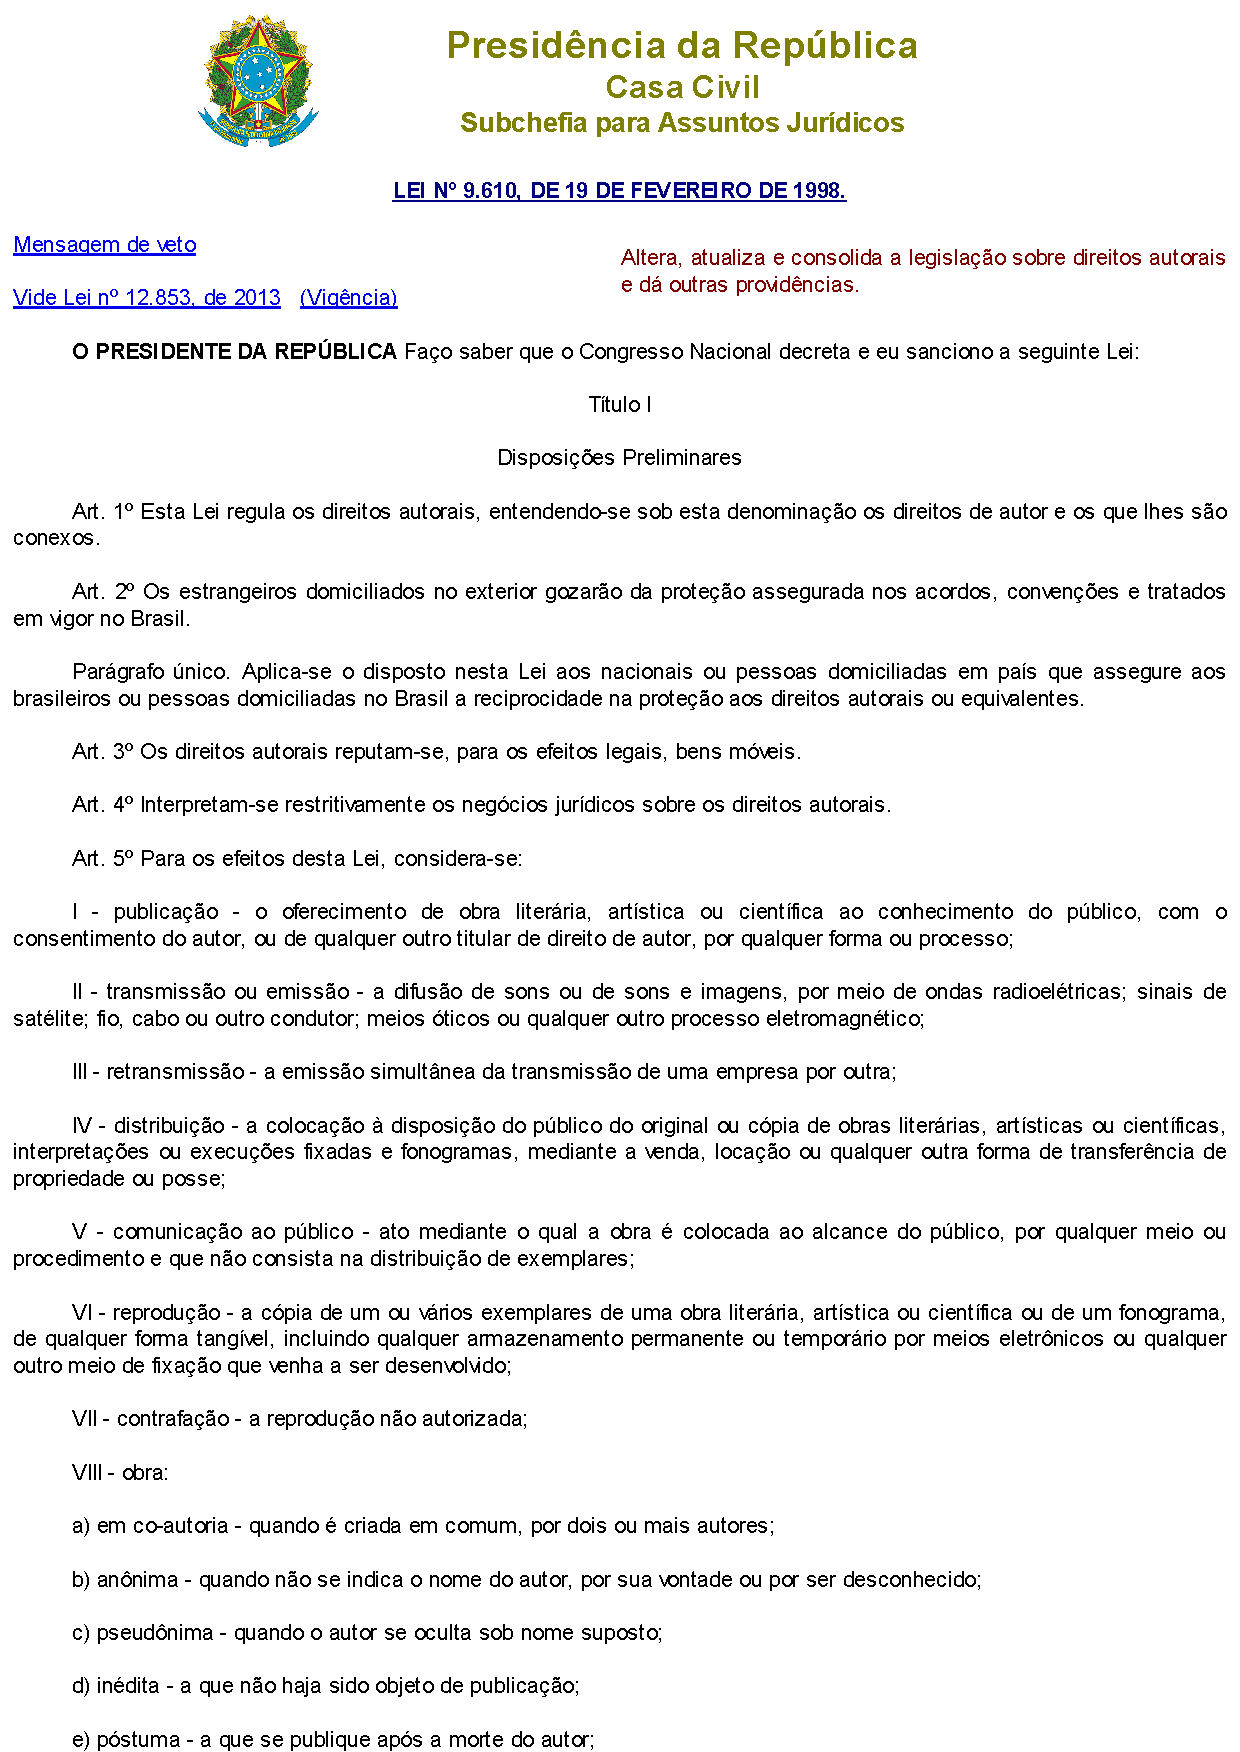
\includegraphics[width=\textwidth]{./PosTexto/Ilustracoes/lei-n9610-p1}}%% Imagem (Dimensões e localização)

\centerline{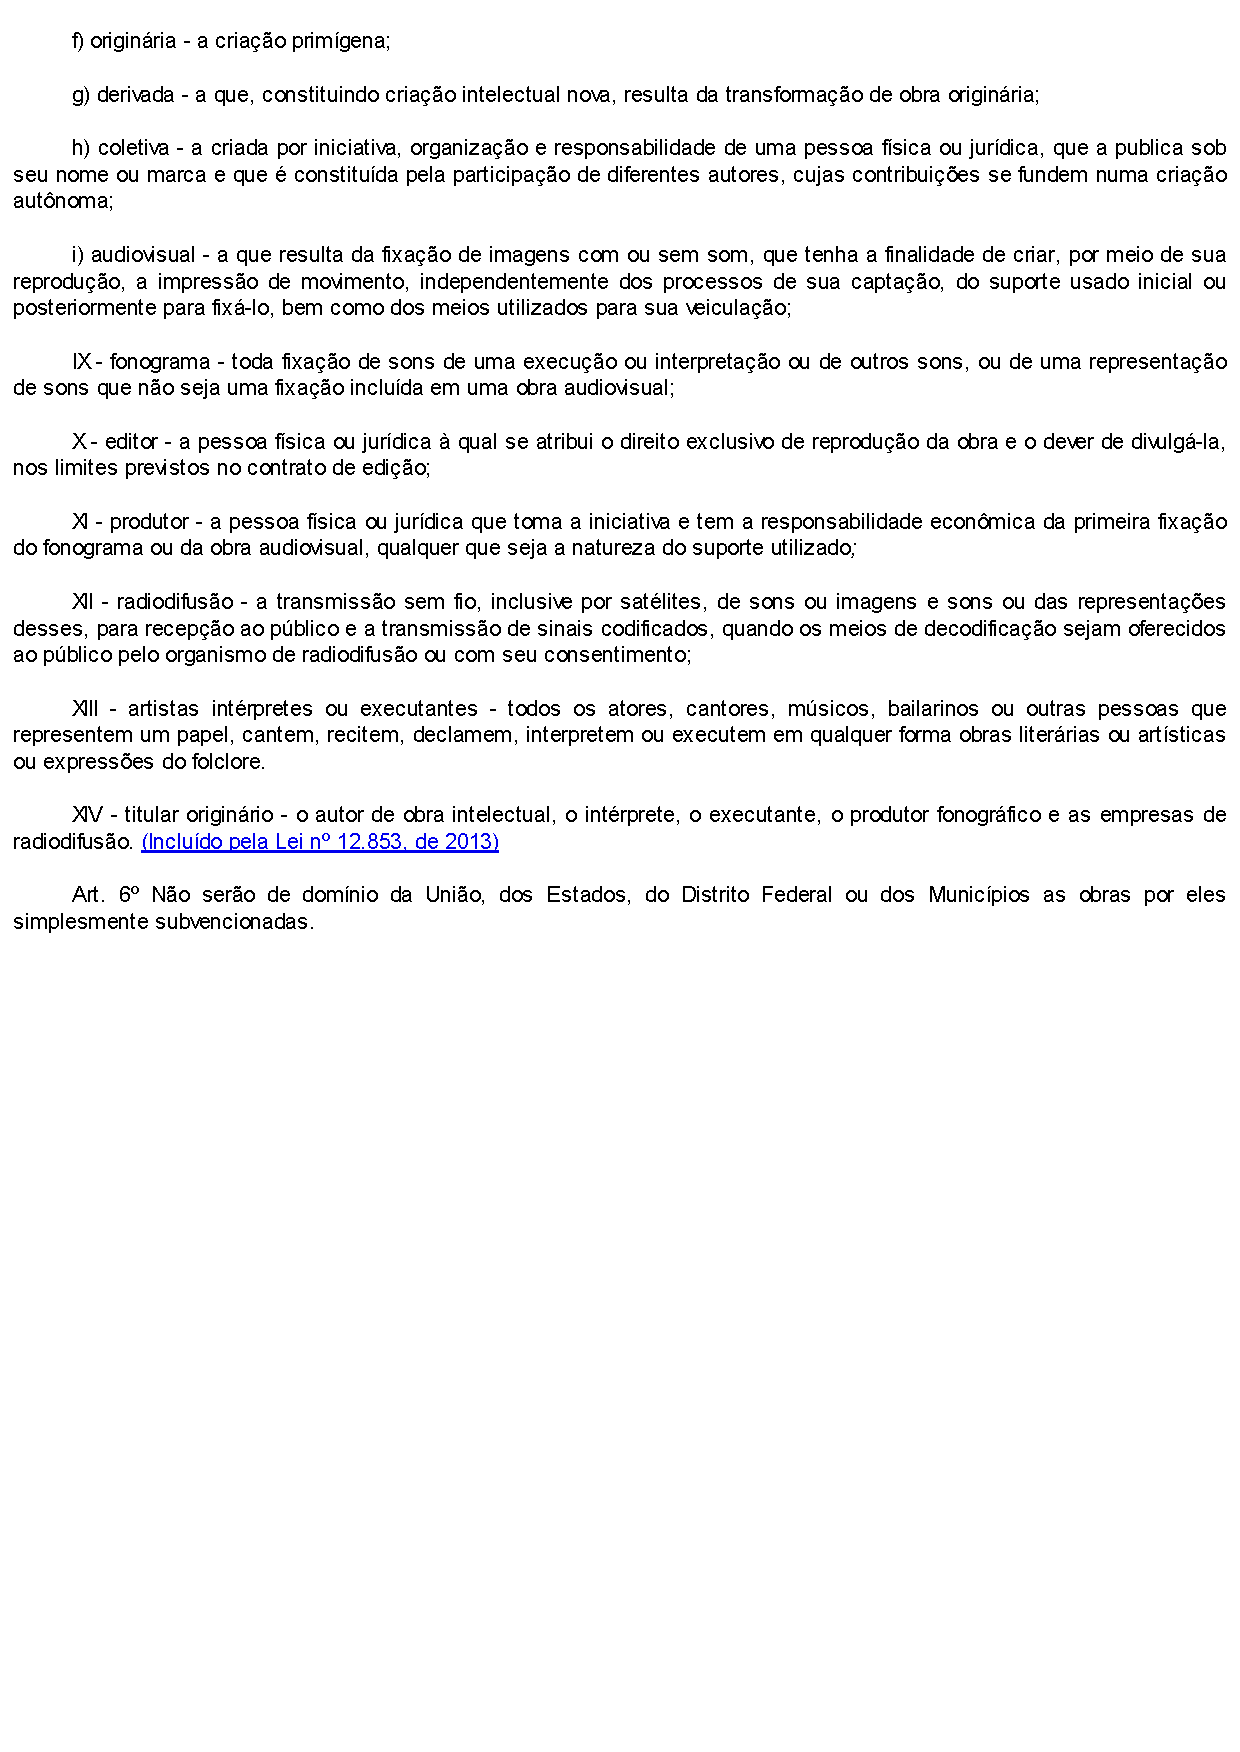
\includegraphics[width=\textwidth]{./PosTexto/Ilustracoes/lei-n9610-p2}}%% Imagem (Dimensões e localização)
%% Anexo - Comente para remover este item
  %%%%% ANEXO B
%%
%% Texto ou documento não elaborado pelo autor, que serve de fundamentação, comprovação e ilustração.

%% Título e rótulo de anexo (rótulos não devem conter caracteres especiais, acentuados ou cedilha)
\chapter{Normas para Elaboração de Trabalhos Acadêmicos}\label{cap:anexob}

As normas da \gls{utfpr} podem ser acessadas em: \url{http://portal.utfpr.edu.br/biblioteca/trabalhos-academicos/discentes/orientacao-para-trabalhos-academicos}. Ver Figura \ref{fig:capadolivro}.

\begin{figure}[htb]%% Ambiente figure
\captionsetup{width=0.9\textwidth}%% Largura da legenda
\caption{Sítio: Normas para Elaboração de Trabalhos Acadêmicos.}%% Legenda
\label{fig:capadolivro}%% Rótulo
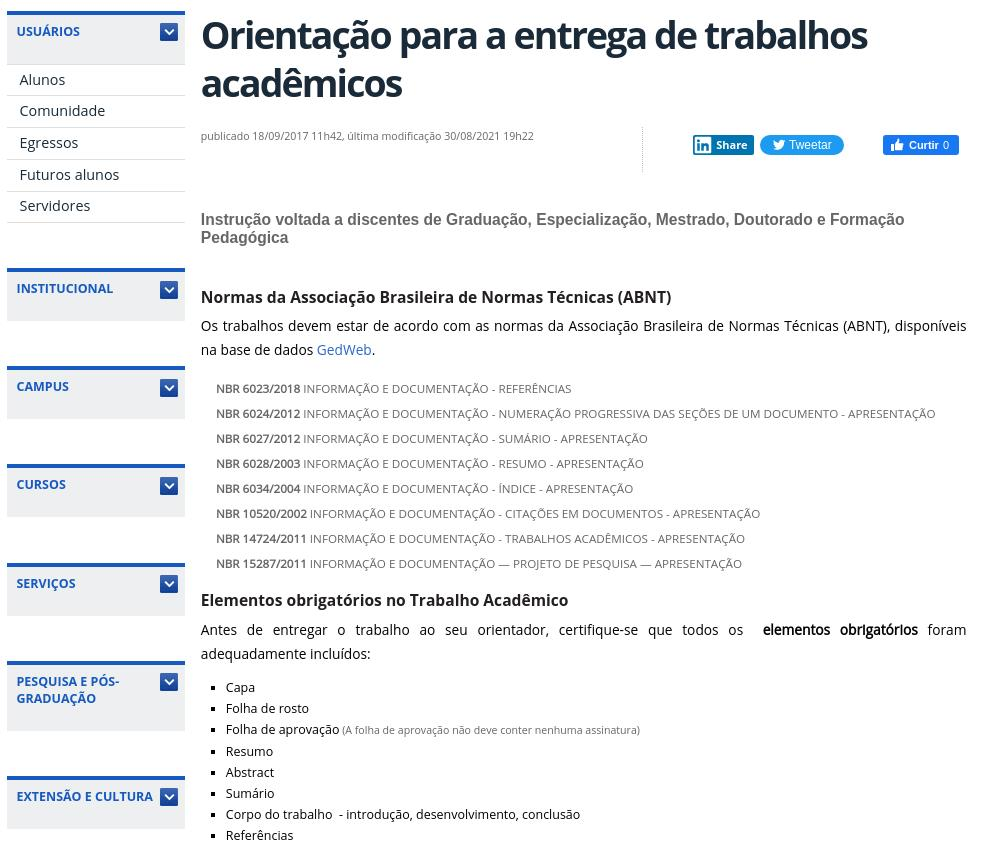
\includegraphics[width=0.9\textwidth]{normas}%% Dimensões e localização
\fonte{\cite{UTFPR2008}}%% Fonte
\end{figure}

%% Anexo - Comente para remover este item
\end{arquivosdeanexos}%% Não comente esta linha

%% Índice - Adiciona um índice remissivo.
%\incluirindice%% Comente para remover este item

%% Fim do documento
\end{document}%% Não comente esta linha
